\chapter{Machine learning theory}
Artificial intelligence can be defined as the discipline that formally describes and characterizes systems that aim to mimic the intelligence and the behavioural patterns of humans. Artificial intelligence involves a set of different disciplines and techniques that overlap in a non-trivial way.

\begin{figure}[H]
                \centering
                        \includegraphics[width=0.45\textwidth]{pics/AI/venn1.png}            \includegraphics[width=0.45\textwidth]{pics/AI/venn2.png}
                        \caption{Two possible venn diagrams for disciplines/techniques involved in the artificial intelligence}
\end{figure}
\noindent A definition of the term "\textbf{Learning}" in relation to algorithms was formulated by \textbf{Tom mitchell} in 1997:
 \begin{adjustwidth}{25mm}{25mm}
                 \rule[0.1cm]{12cm}{0.6mm}\\
                    \textit{"A computer program is said to learn from \textbf{experience} $E$ with respect to some class of \textbf{tasks} $T$ and \textbf{performance} measure $P$, if its performance at task in $T$, as measured by $P$, improves with the experience $E$"  
                    %(represented by the sets of k shingles that each signature represent)
                    }\\
        \rule[0.1cm]{12cm}{0.6mm}\\
\end{adjustwidth}
There are \textbf{three} main \textbf{paradigms} of machine learning approaches, which may contain more specific subcategories :\begin{itemize}
    \item \textbf{Supervised Learning:} in supervised learning techniques the \textbf{ground truth} is known for each training sample. Samples that are labeled with the ground truth are used to tune (\textbf{train}) the parameters of the model. It's common to implement an error function (to be minimized) that measures the difference between the outcome of the model and the ground truth. Once that the training is finished, the resulting model can be used to estimate the labels to be associated with new input data (that doesn't belong to the training set). 
    \begin{figure}[H]
                \centering
                        \includegraphics[width=0.55\textwidth]{pics/AI/supervised.png} 
                        \caption{Supervised learning model schema. The training samples $x$ are coupled with the ground truth $y$}
\end{figure}
    \item \textbf{Unsupervised Learning}: in this kind of techniques there is \textbf{no knowledge} about any \textbf{label} or \textbf{ground truth}. In this approach the model is trained and used to discover patterns and relationship between samples on the basis of some of their intrinsic properties of the data. Once the data have been analysed and grouped according to the criteria imposed by the model, a supervision phase usually follows during which the data are labelled.
    
    \begin{figure}[H]
                \centering
                        \includegraphics[width=0.55\textwidth]{pics/AI/unsupervised.png} 
                        \caption{Unsupervised learning model schema}
\end{figure}
    \item \textbf{Reinforcement learning}:
    this is an area of machine learning concerned with how intelligent agents ought to take actions in an environment in order to maximize the notion of cumulative reward. In order to achieve this, the training \footnote{\href{https://ieeexplore.ieee.org/abstract/document/9244647}{IEEE 9244647}}
     of the model/algorithm is performed by defining a reward and a penalty that are delivered so as to induce the system to make some choices rather than others.
    \begin{figure}[H]
                \centering
                        \includegraphics[width=0.55\textwidth]{pics/AI/reinforcement.png} 
                        \caption{Reinforcement learning model schema}
\end{figure}
\end{itemize}
As we said, there are also some noteworthy sub-categories.\\
The \textbf{Semi-supervised learning} approach deals with a small amount of labeled data and a large amount of unlabeled data. The labeled portion of data is used to train a \textbf{pre-model}: this one will be used to label the unlabelled portion of data. Once that this step is completed, all data, both those originally labelled and those labelled by the pre-model, are used for \textbf{supervised learning} of the definitive predictive model.
\begin{figure}[H]
                \centering
                        \includegraphics[width=0.7\textwidth]{pics/AI/semisupervised.png} 
                        \caption{Semi-supervised learning model schema}
\end{figure}
\noindent Semi supervised learning can be considered a hybrid version of the supervised and unsupervised approach. It can also be considered a specific case of \textbf{weak supervised learning}.\\
\textbf{Weak supervised learning} is a branch of machine learning where noisy, limited, or imprecise sources are used to provide supervision signal for labeling large amounts of training data in a supervised learning setting, alleviating the burden of obtaining hand-labeled data sets.\\
\textbf{Self-supervised learning} approach is a technique that allows to handle a very heterogeneous set of tasks. The idea behind this approach is to \textbf{automatically} generate a \textbf{supervisory signal} which is used to solve some tasks (learning the representation of the data, labelling a dataset etc). In different use cases it's common to start with a small labelled dataset and a larger unlabelled dataset which is used with the help of the supervision signal. In anomaly detection tasks the \textbf{auto-encoding system} is a good example of the usage of this techinque: in this approach there are two functions (\textbf{encoder} and \textbf{decoder}) that can be used to extract a small feature vector from a bigger data point (e.g. an image) and vice-versa. The differences between the original data point and the encoded-decoded data point can be considered potential anomalies.
\begin{figure}[H]
                \centering
                        \includegraphics[width=0.7\textwidth]{pics/AI/selfsuper1.png} 
                                                \includegraphics[width=0.7\textwidth]{pics/AI/selfsuper2.png} 
                        \caption{Auto-encoding anomaly detection system. The reconstructed input can be considered a supervisory signal}
\end{figure}

\section{Fundamentals}
In this section will be introduced some key concept through a regression problem used as example, that is a generalization of the problem discussed in section 2.2.2. Now, consider the following assumptions:\begin{itemize}
    \item We observe a real value $x$ and we wish to use these observation to predict the outcome of a real value target variable $t$,
    \item We are given a training set comprising $N$ observations of $x$, let's say $X\equiv\{x_1...x_N\}$ together with the corresponding outcome of $t$, denoted by $T\equiv\{t_1...t_N\}$
\end{itemize}
The goal is to \textbf{generalize over new unknown observations} the knowledge that we already have over the observed data. We can start by finding a polynomial function that fits our observations. The goal function will have the following shape:
\begin{eqwbg}
y(x,\overline{w})=w_0+w_1x+w_2x^2+...+w_Mx^M=\sum_{j=0}^{M}w_jx^j
\end{eqwbg}
This polynomial function must be the one that minimize a given \textbf{error function} $E$, for example:
\begin{eqwbg}
E(\overline{w})=\sum_{n=1}^{N}[y(x_n,\overline{w})-t_n]^2
\end{eqwbg}
The previous error function is a common one widely used, which is the \textbf{sum of squares} of the difference between the \textbf{predictions} based on $x_n$ (the outcome of the polynomial function) and the corresponding target value $t_n$. Thus we can also choose 
\begin{eqwbg}
E_{RMS}(\overline{w})=\sqrt{2E(\overline{w})/N}
\end{eqwbg} Called \textbf{Root-Mean-Square} error, that is a normalization of the sum of squares.
For this choice of $E$, the minimum respect $\overline{w}$ has an unique solution (the derivative is linear) which can be found in closed form: let's call that solution $\overline{w^*}$. Keep in mind the initial goal: finding this function is not the definitive result but it is just an attempt for the \textbf{generalization task}. In the end, the real performances are evaluated over data that are not necessarily present in the initial observations.
\subsection{Model complexity and hyperparameters}
A key decision to be made is to choose the order $M$ of the polynomial. In this example $M$ governs the number of free parameters,that is the \textbf{complexity of the model}. A fundamental, cross-cutting concept in artificial intelligence is the \textbf{overfitting}: this is a side effect that occurs in models with a complexity too high.
\begin{figure}[H]
                \centering
                        \includegraphics[width=0.8\textwidth]{pics/AI/fitting.png} 

                        \caption{Fitting data points with polynomials of different degrees. The points in black represents the $t_n$ target values}
\end{figure}
 \noindent A model that overfits usually has low/no errors over the set used to tune its parameters (\textbf{training set}) but it has poor performances over data never seen before, that means that it fails in generalizing the results obtained during the training: a system that overfits cannot be used to predict anything.
 \begin{figure}[H]
                \centering
                        \includegraphics[width=0.6\textwidth]{pics/AI/overfit.png} 

                        \caption{The overfitting problem}
\end{figure}
\noindent The over-fitting phenomenon can be handled without sacrificing the complexity of the model: a common technique is to introduce a \textbf{regularization hyperparameter}. For example, in our case we can modify the error function $E$ as follows:
\begin{eqwbg}
E_{\lambda}(\overline{w})=\sum_{n=1}^N[y(x_n,\overline{w})-t_n]^2+\frac{\lambda}{2}\norm{\overline{w}}^2
\end{eqwbg}
Where $\lambda$ is the \textbf{hyperparameter}. This new error function adds a penalty which makes the error to grows as the number of the model parameters increases. An \textbf{hyperparameter} is a parameter that is fixed before to start the training step during which it remains constant. It's common to  train the same model with different values of the same hyperparameter in order to see how performances varies
\subsection{Dataset partitions}
As we said, real performances are evaluated over data that could be \textbf{unseen} during the training. Moreover, it's common to train different models with the \textbf{hyperparameters} tuned differently , which must then be compared before testing the final performances using a further dataset. 
For these reasons and others, if the dataset is \textbf{plentiful}, it can be partitioned in different subsets where each one has to accomplish a specific phase. A standard dataset partition consist in 3 subsets:\begin{itemize}
    \item \textbf{Training set}:  training set is the subset used to tune the free parameters of the model (in our example, $\overline{w}$). A supervised learning algorithm looks at the training dataset to determine, or learn, the optimal combinations of variables that will generate a good predictive model,
    
    \item \textbf{Validation set}, also said \textbf{dev set}: the validation set is used to tune the hyperparameters of the model. It can also be used to compare the performances of different models that passed the training phase while being initialized with a different fixed hyperparameter.
    
                \item \textbf{Test set}: the test set is used for the final evaluation of the performances of the model (or a small set of models).
\end{itemize}

 \begin{figure}[H]
                \centering
                     \includegraphics[width=0.6\textwidth]{pics/AI/datasets.png} 
                        \caption{Dataset standard partition}
\end{figure}
\noindent As we said, there are approaches that falls in the \textbf{weak supervised learning} family that allows to handle poor datasets, but there are also some partition techniques that allow to manage this problem upstream at \textbf{dataset level}. A good example is the \textbf{cross-validation} technique. The idea is to choose an integer number $S$, and then to allocate a fraction $1/S$ for the \textbf{validation set} and a fraction $(S-1)/S$ for the \textbf{training set}. We can clearly see that this partition can be done in $S$ different ways: this means that we can make $S$ different \textbf{train-validation-test} runs and then we can \textbf{average} performance scores resulting from different runs.
 \begin{figure}[H]
                \centering
                     \includegraphics[width=0.8\textwidth]{pics/AI/crossval.png} 
                        \caption{Cross validation, $S=5$. This representation is done for simplicity, the proportion between validation and training set does not necessarily have to be the same between different runs.}
\end{figure}
\noindent A limit case occur when we choose $S=N$ ($N$= number of datapoints).
In this case we have $N$ runs in which a \textbf{single datapoint} is used for validation. This is an extrema-ratio applied when dataset is particularly poor. There are some \textbf{drawback} in using the cross validation: the computational feasibility of the single should be taken in account since it's increased by a factor of S. Moreover, if we have multiple hyperparameters, exploring all possible combinations could require, in the worst case, a number of training runs that is exponential with the number of the hyperparameters.
\section{Support Vector Machine (SVM)}
SVM is a method related with the statistical learning theory introduced in 1992 and it is part of the family of \textbf{kernel methods}. It is a \textbf{pattern classification} technique that allows to find a \textbf{separation hyperplane} in the feature space of the data on which it is applied. Data falling within the different defined regions of the hyperplane will be labelled differently.
\begin{figure}[H]
                \centering
                        \includegraphics[width=0.80\textwidth]{pics/AI/svm1.png} 
           
                        \caption{Hyperplanes in two feature spaces feature spaces, respectively in $\R^2$ and $\R^3$}
\end{figure}
\subsection{Introductory concepts}
Suppose having a dataset $\overline{X}=\{\overline{x}_1,\overline{x}_2,\overline{x}_3...\overline{x}_n\}$, where each data point is 2-dimensional and is in the form $\overline{x}_j=(x^{(j)}_1,x^{(j)}_2)^\top$.  We can also indicate the two generic features $x_1,x_2\in\R$ without any superscript and the generic datapoint belonging to $\R^2$ with $\overline{x}=(x_1,x_2)^\top$ without any subscript.\\
Now, let's define the function of the $D-$dimensional space $g(\overline{x})$:
\begin{eqwbg}
g(\overline{x})=w_0+\sum_{i=1}^D w_ix_i
\end{eqwbg}
In our example, $D=2$, then $g(\overline{x})=w_0+w_1x_1+w_2x_2$\\
\noindent The points such that $g(\overline{x})=0$ identify the \textbf{decision surface}. While specifying the function $g(\overline{x}$,  we are doing nothing more than choosing a vector  $\overline{w}=(w_1,w_2)^\top$ and a scalar $w_0$. After choosing them, we can see that:
\begin{eqwbg}
g(\overline{x})=w_0 + \overline{w}^\top\overline{x}
\end{eqwbg}
We can demonstrate that $\overline{w}$ is \textbf{orthogonal to any vector lying} on the decision surface: suppose having 2 generic datapoints $\overline{x}_p,\overline{x}_q$ lying on the decision surface. We can write:
\begin{eqwbg}
\begin{aligned}
  &g(\overline{x}_p)=g(\overline{x}_q)=0 \longrightarrow\\
  &\overline{w}^\top\overline{x}_p +w_0=\overline{w}^\top\overline{x}_q +w_0\longrightarrow\\
  &\overline{w}^\top(\overline{x}_p-\overline{x}_q)=0
\end{aligned}
\end{eqwbg}
\begin{figure}[H]
                \centering                       \includegraphics[width=0.80\textwidth]{pics/AI/svm_intro.png} 
                        \caption{SVM. In this case,  $g(\overline{x})=w_0+w_1x_1+w_2x_2$. The vector $\overline{x}_p-\overline{x}_q$ lying on the green line (\textbf{decision surface}) is orthogonal to $\overline{w}$} 
\end{figure}
\subsection{Geometrical considerations}
We can start considering a generic point $\overline{x}^*$. We can define:\begin{itemize}
    \item $r$: the scalar value representing \textbf{the modulus of the distance vector} between the decision surface $g(\overline{x})=0$, and  $\overline{x}^*$ 
    \item $r_0$: the scalar value representing \textbf{the modulus of the distance vector} between the decision surface $g(\overline{x})=0$, and  the origin of the axis,
    \item $\overline{x}^*_{proj}$: the projection of $\overline{x}^*$ on the decision surface.
    \item $\hat{w}$: the versor of the vector $\overline{w}$, reminding that $\hat{w}=\overline{w}/\norm{\overline{w}}$
\end{itemize}
\begin{figure}[H]
                \centering                       \includegraphics[width=0.80\textwidth]{pics/AI/svm_intro2.png} 
                        \caption{Geometrical considerations for SVM} 
\end{figure}
Remind that, for a given $\overline{x}^*$, the value $g(\overline{x}^*)$ is a \textbf{scalar}, and  $g(\overline{x})=g(\overline{x}^*)$ represent an hyperplane that is \textbf{parallel} to the decision surface.
The previous concepts are represented in figure. Moreover, we can write:
\begin{eqwbg}
\overline{x}^*=\overline{x}^*_{proj}+r\hat{w}
\end{eqwbg}

\subsection{Boundary for linearly separable problems}
Let's start considering an SVM approach in which  data points belong to classes that are \textbf{linearly separable} in the feature spaces. This means that, in general, there will be different \textbf{decision surfaces} that could be chosen to \textbf{classify} the data points. The criteria to choose a decision surface is to choose the one that is as\textbf{ far away from the data} of both classes as possible. We can start by defining these 2 \textbf{hyperplanes}:
\begin{eqwbg}
\begin{aligned}
&g(\overline{x})=\overline{w}^\top \overline{x}+w_0=-1 \quad \textrm{(class 1 surface)}\\
&g(\overline{x})=\overline{w}^\top \overline{x}+w_0=1  \quad \textrm{(class 2 surface)}
\end{aligned}
\end{eqwbg}
Then, we define the \textbf{distance} between these parallel surfaces as $m$, that is, the \textbf{margin}.
\begin{figure}[H]
                \centering                       \includegraphics[width=0.80\textwidth]{pics/AI/svm_intro3.png} 
                        \caption{Representation of the margin $m$} 
\end{figure}
\noindent As shown in fig 4.13, the distance between the origin and an hyperplane in the form $\overline{w}^\top \overline{x} + x_0 = 0$ is given by $r_0=w_0/\left\Vert\overline{w}\right\Vert$. Thus, $m$ can be found as follows:
\begin{eqwbg}
m=\underbrace{\frac{1-w_0}{\left\Vert\overline{w}\right\Vert}}_{\textrm{distance class 2}}-\overbrace{\frac{-(1+w_0)}{\left\Vert\overline{w}\right\Vert}}^{\textrm{distance class 1}}=\frac{2}{\left\Vert\overline{w}\right\Vert}
\end{eqwbg}
That is, the distance between the origin and the  class 2 surface \textbf{minus} the distance between the origin and the class 1 surface.
The best choice of $\overline{w}$ will be the one that maximizes the \textbf{margin} $m$, that means that we wish to \textbf{minimize} $\left\Vert\overline{w}\right\Vert$ constrained to the fact that we' re not performing any \textbf{classification error} (problem is separable for assumption). In order to formalize mathematically this last constraint, consider :\begin{itemize}
    \item  $\overline{X}=\{\overline{x}_1,\overline{x}_2,...\overline{x}_n\}$ is the dataset containing $n$ $D$-dimensional points $\overline{x}_j$;
    \item For each $\overline{x_j}$, we have a  \textbf{class label} $y_j\in \{-1,1\}$
\end{itemize}
A \textbf{decision surface} correctly classifies  all the datapoints of the dataset if the following inequality holds:\[
 y_i(\overline{w}^\top\overline{x}_i+w_0)\geq1 \quad \forall i\in \{1,2...n\}
\]
Thus, in order to perform the best choice of $\overline{w}$, we wish to solve the following problem:\[
\begin{cases}
\textrm{Minimize:} \quad \displaystyle\frac{1}{2}\left\Vert\overline{w}\right\Vert^2\\
\phantom{a}\\
\textrm{While:\phantom{iiize}} \quad  y_i(\overline{w}^\top\overline{x}_i+w_0)\geq1, \quad \forall i\in \{1,2...n\}
\end{cases}
\]
This constrained optimization problem can be solved with the \textbf{Lagrangian multiplier} method:\[
\Lagr=\frac{1}{2}\underbrace{\overline{w}^\top\overline{w}}_{\left\Vert\overline{w}\right\Vert} + \sum_{i=1}^n\alpha_i(1-y_i(\overline{w}^\top\overline{x}_i+w_0))
\]
Setting the gradient with reference to $\overline{w}$ and $w_0$ to be $0$, we have\[
\overline{w}-\sum_{i=1}^n\alpha_iy_i\overline{x_i}=\overline{0}\implies\begin{cases}
\displaystyle\sum_{i=1}^n\alpha_iy_i\overline{x}_i=\overline{w},\\
\phantom{a}\\
\displaystyle\sum_{i=1}^n\alpha_iy_i=0
\end{cases}
\]

\noindent Substituting the result obtained for $\overline{w}$ in the lagrangian multiplier, we obtain constrained function of $\overline{\alpha}=\{\alpha_1,\alpha_2...\alpha_n\}$ that we wish to \textbf{maximize}:\[
\begin{cases}
\textrm{Maximize:}\quad \displaystyle\mathcal{W}(\overline{\alpha})=\sum_{i=1}^n\alpha_i-\frac{1}{2}\sum_{j=1}^n\sum_{k=1}^n\alpha_j\alpha_k\underbrace{y_jy_k\overline{x}^\top_j\overline{x}_k}_{\substack{\textrm{Known} \\ \textrm{from}\\ \textrm{dataset}}};\\
\phantom{a}\\
\textrm{While:\phantom{iiize}}\quad\alpha_i\geq0,\quad \forall i\in \{1,2,...n\}\\
\textrm{\phantom{Whileiiize:}}\quad\displaystyle\sum_{i=1}^n\alpha_iy_i=0,\quad \forall i\in \{1,2,...n\}
\end{cases}
\]
A global maximum of $\overline{\alpha}$ can always be found, then we can recover $\overline{w}$ from the 4.14. After that we've found $\overline{w}$, we can obtain $w_0$ using the following relation:\[
\begin{aligned}
\frac{1}{n}\sum_{i=1}^ny_i(\overline{w}^\top x_i&+w_0)=1\\
&\Downarrow\\
w_0=\frac{1}{n}\sum_{i=1}^n&y_i-\overline{w}^\top x_i
\end{aligned}
\]
That is, we're averaging  $w_0$ for all the datapoints using the equation that defines the two class surfaces given the decision surface($\overline{w}$).\\
There are different \textbf{algorithms} that can be used to build the SVM. It's important to understand that each $\alpha_i$ is associated to a datapoint for which it represent the information about the "\textbf{weight}" of that datapoint in the calculation of the \textbf{decision surface}. Only a small subset of the datapoints will have an $\alpha_i>0$, i.e. the \textbf{nearest} to the margin. These datapoint are called \textbf{support vectors} (hence, the name of the technique) and are the only involved in finding the \textbf{decision surface}.
\subsection{Non-linearly separable problems}
If we're dealing with a non-linearly separable problem, for each datapoint $x_i$ we need to introduce a \textbf{slack variable}, denoted with $\xi_i$. The \textbf{slack variablie} quantifies the distance of $x_i$ from the correct \textbf{class surface}.
\begin{figure}[H]
                \centering                       \includegraphics[width=0.80\textwidth]{pics/AI/svm_intro4.png} 
                        \caption{Slack variable for the 2 points $\overline{x}_j$ and $\overline{x}_i$. Remember that $m=\displaystyle\frac{2}{\nrm{\overline{w}}}$} 
\end{figure}
\noindent For example , for the generic point $\overline{x}_i$ (Figure 4.15) we can write:\[
\begin{aligned}
\xi_i=1-y_ig(\overline{x_i})
\end{aligned}
\]
The outcome of a generic $\xi_i$ gives us information about the goodness of the classification of $\overline{x_i}$:
\[
\begin{cases}
\xi_i=0 \phantom{>i1}\implies\quad \textrm{ correct classification},\\
0<\xi_i<1 \implies\quad \textrm{ correct classification but inside the margin},\\
\xi_i\geq1\phantom{>i1}\implies\quad\textrm{ missclassification}
\end{cases}
\]
The case $\xi_i<0$ is not considered: only datapoints with $\xi_i\geq0$ contribute to the linear non-separability of the problem. 
Thus :\[
\begin{aligned}
&\#\{\xi_i>0\}\quad\implies\quad\textrm{number of non-separable points}\\
&\#\{\xi_i>1\}\quad\implies\quad\textrm{number of missclassifications}
\end{aligned}
\]
It's clear that the value $\sum_i\xi_i$ should be minimized.
Therefore, after that we ve introduced the \textbf{slack variables} the problem  written in 4.12 become:\[
\begin{cases}
\textrm{Minimize:} \quad \displaystyle\frac{1}{2}\nrm{\overline{w}}^2+ C\sum_{i=1}^n\xi_i\\
\phantom{a}\\
\textrm{While:\phantom{iiize}} \quad  y_i(\overline{w}^\top\overline{x}_i+w_0)\geq1-\xi_i, \quad \forall i\in \{1,2...n\}
\end{cases}
\]
$C$ is the \textbf{tradeoff hyperparameter} between error and margin. The choice of $C$ is critical: if it's not tuned properly \textbf{over/under-fitting} may incur. Usually several possible choices of $C$ are found empirically using different subsets of the dataset, then the value that performs best during \textbf{validation} step is chosen. The hyperplane found solving this problem is called \textbf{soft margin hyperplane}
\subsection{Data transformation}
Problems that are non linearly separable can be made separable \textbf{mapping} the feature space in an highest dimensional space\footnote{\textit{Cover's theorem}, \href{https://en.wikipedia.org/wiki/Cover\%27s_theorem}{wiki} and \href{https://web.archive.org/web/20191220234502/http://pdfs.semanticscholar.org/445a/d69010658097fc317f7b83f1198179eebae8.pdf}{paper}}.
The idea is to increase the dimension of the data point in this way:  one or more features are \textbf{mapped}  in another space and then \textbf{added} to the data point.
\begin{figure}[H]
                \centering                       \includegraphics[width=0.80\textwidth]{pics/AI/coversep.png} 
                        \caption{Example of a feature mapped in a polynomial space turning a non linearly separable problem into a separable one} 
\end{figure}
\noindent There are different basis that could be used. While considering a feature $x_k$, in SVM the basis most commonly used are:\begin{itemize}
    \item \textbf{Polynomial}: polynomial terms of $x_k$,
    \item \textbf{Radial basis functions}: gaussian-like:\[
    \phi(x_k)=e^{-\frac{|x_k-c|^2}{\sigma^2}}
    \]
    \item \textbf{Sigmoid functions} of $x_k$:\[
    \sigma(x_k)=\frac{1}{1+e^{-x}}
    \]
\begin{figure}[H]
    \centering
    \begin{tikzpicture}
	\begin{axis}[
		xlabel=$x_k$,
		ylabel={$\sigma(x_k)$}
	]
	    \addplot[mark=none,color=red,domain=-8:8] {1/(1+e^(-x))};
	    \end{axis}
    \end{tikzpicture}                        
    \caption{Sigmoid function} 
\end{figure}
    
\end{itemize}
Keep in mind that, without loss of generality, we can apply different \textbf{transformations} to the different \textbf{features} of the datapoint even using functions belonging to different \textbf{families}. We shall indicate the \textbf{ensemble} of the transformations applied to a datapoint with $\eta(\overline{x})$.
Once that we have chosen an $\eta(\overline{x})$, we can define the \textbf{Kernel function} $K(\overline{x}_i,\overline{x}_k)$ as
\[
K(\overline{x}_i,\overline{x}_k)=\eta(\overline{x}^\top_j)\eta(\overline{x}_k)
\]
Therefore we can modify the $\mathcal{W}(\alpha)$ appearing in the 4.15 as follow:
\[
\begin{aligned}
\mathcal{W}(\overline{\alpha})=\sum_{i=1}^n&\alpha_i-\frac{1}{2}\sum_{j=1}^n\sum_{k=1}^n\alpha_j\alpha_ky_jy_k\overline{x}^\top_j\overline{x}_k\\
&\Downarrow \textrm{We define  }\eta(\overline{x}) \Downarrow\\
\mathcal{W}(\overline{\alpha})=\sum_{i=1}^n\alpha_i&-\frac{1}{2}\sum_{j=1}^n\sum_{k=1}^n\alpha_j\alpha_ky_jy_kK(\overline{x}_j,\overline{x}_k)\\
\end{aligned}
\]
\noindent The term $K(\overline{x}_j,\overline{x}_k)$ can be \textbf{pre-calculated} and stored in a matrix. This is called the \textbf{Kernel trick optimization}.
\section{Outlier detection}
\textbf{Outlier} detection is  a \textbf{decision} problem. There is no rigid mathematical definition of what constitutes an \textbf{outlier}; determining whether or not an observation is an outlier is ultimately a subjective exercise. We can describe it as follow:
 \begin{adjustwidth}{25mm}{25mm}
                 \rule[0.1cm]{12cm}{0.6mm}\\
                    \textit{In statistics, an \textbf{outlier} is a data point that differs significantly from other observations. An outlier may be due to variability in the measurement or it may indicate experimental error.}\\
        \rule[0.1cm]{12cm}{0.6mm}\\
\end{adjustwidth}
The \textbf{background scenario} plays a key role as in many \textbf{decision} problems: there are scenarios in which outliers represents anomalies (\textbf{anomaly detection} task) that should be monitored, but there are other scenarios in which outliers represents non-relevant data. The trickiest part of the task is to distinguish  \textbf{ordinary} low probability events/items from \textbf{real outliers}. In the following sections, we'll describe some \textbf{outlier detection methods}, before starting we'll assume that :\begin{itemize}
    \item We have a set of samples $\overline{X}^*=\{\overline{x}_i\}$;
    \item $N = \dim(\overline{X}^*)$ is the dimension of the set;
    \item $D = \dim(\overline{x}_i)$ is the dimension of the samples that belong to $\overline{X}^*$
\end{itemize}
Classic methods that will be described shortly aim to \textbf{decide} whether any $\overline{x}_i$ can be considered an \textbf{outlier} or or not.
\subsection{Inter Quartile Range detection}
\textbf{IQR-based} detection is a \textbf{data-driven}, \textbf{component-wise} outlier detection method:  this method is  applied to each one of the D dimension of the samples belonging to our data set. Thus, for each scalar component we compute the \textbf{first quartile} $Q_1$ and the \textbf{third quartile} $Q_3$, then we compute and the difference $IQR=Q_3-Q_1$.
All values which \textbf{don t} fall in the range $[\,Q_1-k(IQR),\;Q_3+k(IQR)\,]$ are considered \textbf{outliers}. The $k$ is a chosen \textbf{hyperparameter} ($k=1.5$ is common).

\begin{figure}[H]
\centering
                        \includegraphics[width=\textwidth]{pics/IQR.png}
\caption{Graphical representation of the IQR range detection method. Samples that fall in the green range are considered regular, otherwise they are considered outliers}
\end{figure}

\subsection{Elliptic envelope}
\textbf{Elliptic envelope} is a \textbf{model based} outlier detection method. This method is applied to the whole observation $\overline{x}_i$ and not \textbf{component-wise}. It starts by assuming a \textbf{multivariate ditribution} model for the $\overline{x}_i$ data points. The methods is valid for any multi variate distribution in any dimension, but for simplicity let's suppose having $D=2$ and consider a \textbf{gaussian} multi variate distribution model. \\We have to define  the \textbf{contamination} hyperparameter, let's call it $\eta\mid\, \frac{1}{10} \leq \eta \leq \frac{1}{2}$. This value represent the \textbf{fraction of the outliers} that are present in the dataset. Not knowing priorly the exact proportion of the outliers in the dataset is the major limitation of using this method. \\
All the samples falling in the tail volume of the model which enclose the $\eta$ percent of the total volume (N.B. the distributions always integrates to 1) \textbf{are considered outliers}. Thus, in the multivariate gaussian example,  the $\eta$  unambiguously defines \textbf{an ellipse} within which the samples are considered \textbf{regular}

\begin{figure}[H]
\centering
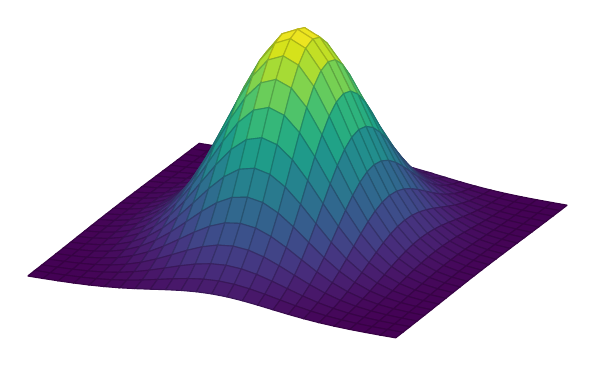
\begin{tikzpicture}
\begin{axis}[
    colormap/viridis,
  	hide axis
]
\addplot3[
    surf,
]
{(exp(-(x^2)/5-(y^2)/9))*1/4};
\end{axis}
\end{tikzpicture}
\centering
                        \includegraphics[width=200px]{pics/ellenv.png}
\caption{Representation of an ellipse (right) defined by an hyperplane intersecting the multi variate gaussian (left). Green samples are regular, red ones are outliers}
\end{figure}




\section{Dimensionality reduction}
Dimensionality reduction is a common task while dealing with datasets. It can be helpful for different reasons: time/space complexity reduction,  simpler models can be built, observability of the dataset is increased and so on. Suppose that we have datapoints with $d$ feature. If we want to reduce them to $k$ feature, we can just discard $d-k$ (\textbf{feature selection}) or we can project the original $d$ dimension to a new space with $k$ dimensions (\textbf{feature  extraction}).
Dimensionality reduction can be performed while considering the class associated to each datapoint (\textbf{supervised} or not (\textbf{unsupervised}).
\subsection{Principal Component Analysis (PCA)}
\textbf{PCA} is an \textbf{unsupervised} dimensionality reduction technique. The idea behind this method is to project datapoints into a slower-dimension space while \textbf{minimizing} the information loss. Now, consider the following assumptions:\begin{itemize}
    \item We have a dataset $\overline{X}=\{\overline{x}_1,\overline{x}_2...\overline{x}_n\}$ of $n$ datapoints, 
    \item The \textbf{dimension} of the generic datapoint $\overline{x}$ is  $\textrm{dim}(\overline{x})=d $,
    \item We wish to reduce dimension from $d$ to $k$, with $k<d$.
\end{itemize}
Therefore, we can consider the projection of $\overline{x}$ in the new space as $\overline{z}$:\[
\overline{z}=\overline{W}^\top\overline{x}
\]
Where $\overline{W}$ is  the \textbf{projection matrix}. Remember that:\[
\begin{aligned}
&\textrm{dim}(\overline{x})=d\\
&\textrm{dim}(\overline{z})=k\\
&\textrm{dim}(\overline{W})=d \times k
\end{aligned}
\]The resulting projected dataset is indicated with $\overline{Z}=\{\overline{z}_1,...\overline{z}_n\}$. The projection matrix that maximizes the \textbf{sample variance} of the dataset $Var(\overline{Z})$ is the one that minimize the \textbf{information loss}. \\ Indicating with $\overline{M}_x$ the \textbf{sample mean} of the dataset $\overline{X}$ and (with misuse of notation) with $\overline{W}^\top\overline{X}$,  the \textbf{projection} of each datapoint $\overline{x}_i\in\overline{X}$ in the new space $\overline{Z}$,we can write :\[
\begin{aligned}
Var(\overline{Z})&=Var(\overline{W}^\top\overline{X})=E\left[(\overline{W}^\top\overline{X}-\overline{W}^\top\overline{M}_x)^2\right]\\
&=E\left[\overline{W}^\top(\overline{X}-\overline{M}_x)(\overline{X}-\overline{M}_x)^\top\overline{W}\right]\\
&=\overline{W}^\top \underbrace{E\left[(\overline{X}-\overline{M}_x)(\overline{X}-\overline{M}_x)^\top\right]}_{\substack{\displaystyle\Sigma_x\\\textrm{(Covariance matrix of $\overline{X}$)}}}\overline{W}\\
\end{aligned}
\]
Remember that the \textbf{covariance matrix} represent the \textbf{variance} of a \textbf{multi-dimensional} random variable (or the \textbf{sample} variance of a set of \textbf{observations}, i.e. a dataset).
Thus, we can formalize the goal of the \textbf{PCA} as:\[
\begin{cases}
\textrm{Maximize:}\quad Var(\overline{Z})\\
\textrm{Subject to:} \quad \nrm{\overline{W}}=1
\end{cases}
\]
Now consider the vector $\overline{w}_1 \mid \textrm{dim}(\overline{w}_1)=k$ for which it holds:\[
\Sigma_x\overline{w}_1 = \lambda_1w_1
\]
Thus, $\overline{w}_1$ is an \textbf{eigenvector} for $\Sigma_x$ with $\lambda_1$ as \textbf{eigenvalue}. The eigenvector associated with the largest eigenvalue is the one along whose direction the dataset has the \textbf{highest variance}, therefore the loss of information is minimal. Thus, we can procedurally choose \textbf{eigenvectors} with decreasing \textbf{eigenvalues} (starting from the greatest) as the new basis for the space onto which we want to project the dataset. Considering that $\Sigma_x$ has $d$ eigenvectors and we have to pick the $k$ ones with the \textbf{greatest eigenvalues}, a key aspect is to evaluate how to choose $k$. A metric related to this aspect is the \textbf{Proportion of Variance Explained}, indicated with $\mathcal{P}_v$. If we consider \[
\begin{aligned}
\lambda_1>\lambda_2...>\lambda_d
\end{aligned}
\]Then $\mathcal{P}_v$  can be computed as:\[
\mathcal{P}_v=\frac{\overbrace{\lambda_1+\lambda_2+...\lambda_k}}{\underbrace{\lambda_1+\lambda_2+...\lambda_k}+\lambda_{k+1}+...\lambda_d}
\]
Typically, $k$ is chosen so as to have $\mathcal{P}_v \geq 0.9$.
\begin{figure}[H]
                \centering                       \includegraphics[width=0.80\textwidth]{pics/AI/pov.png} 
                        \caption{Eigenvectors and eigenvalues in decreasing order (a) and the value of $\mathcal{P}_v$ (b) plotted in function of $k$ (number of eigenvectors chosen for the new basis)} 
\end{figure}
\subsection{Fisher Linear Discriminant Analysis (LDA)}
\textbf{Fisher LDA} is a \textbf{supervised}   dimensionality reduction technique. In this section will be shown an example of application of \textbf{LDA} on a 2-dimensional space projected into a mono-dimensional space, but the procedure is also valid from $d$ to $k$ dimension, with $d>k$. 
Now, lets'start considering:\begin{itemize}
    \item $\overline{X}=\{(\overline{x}_i, c_i)_i\}$, with $i=1...n$ is the \textbf{dataset} made of  $n$ couples;
    \item For each couple $(\overline{x}_i, c_i)_i$ we have $\overline{x}_i \in \R^2$ which is the \textbf{observation} (datapoint) and $c_i$ which is the \textbf{class label};
    \item We have 2 possible classes $C_1$ and $C_2$. Thus, for each observation-label pair, it holds:\[
    \begin{cases}
        \overline{x}_i \in C_1\quad\longrightarrow c_i=1\\
        \overline{x}_i \in C_2 \quad \longrightarrow c_i=0 
    \end{cases}
    \]
    \item The \textbf{means} of the two sets of datapoints belonging to $C_1$ and $C_2$ are respectively $\overline{\mathcal{M}}_1$ and $\overline{\mathcal{M}}_2$.
    
\end{itemize}
The key idea behind the \textbf{LDA} is to project datapoints $\overline{x}_i$ into a new space in which the the distance between \textbf{class averages} is maximized and the \textbf{variance} of each class is minimized: with these 2 criteria we ensure that we can \textbf{distinguish} as easily as possible points belonging to different classes. Therefore, consider:\begin{itemize}
        \item $z=\overline{w}^\top\overline{x}$ is the generic datapoint projected in a \textbf{monodimensional} space, with $\overline{w}$ as \textbf{projection vector},
        \item In this new space, the \textbf{means} of the two sets of datapoints belonging to $C_1$ and $C_2$ become $\mu_1$ and $\mu_2$,
        \item In this new space, we indicate with $\sigma_1^2$ and $\sigma_2^2$, the \textbf{variances} of the two set of datapoints belonging to $C_1$ and $C_2$ respectively
    \end{itemize}
\begin{figure}[H]
                \centering                       \includegraphics[width=0.80\textwidth]{pics/AI/LDA.png} 
                        \caption{Representation of \textbf{LDA} applied for a 2-dimensional space turning into a mono-dimensional space} 
\end{figure}
Thus, we can compute:\[
\begin{aligned}
&\sigma_1^2=\sum_{\overline{x}_i\in C_1}(\overline{w}^\top\overline{x}_i-\mu_1),\quad \sigma_2^2=\sum_{\overline{x}_i\in C_2}(\overline{w}^\top\overline{x}_i-\mu_2),\\
&\phantom{aaa}\\
&\mu_1=\frac{\displaystyle\sum_{\overline{x}_i\in C_1}\overline{w}^\top \overline{x}_i}{\displaystyle\sum_{\overline{x}_i\in C_1}c_i},\phantom{aaaaaaa}
\mu_2=\frac{\displaystyle\sum_{\overline{x}_i\in C_2}\overline{w}^\top \overline{x}_i}{\displaystyle\sum_{\overline{x}_i\in C_2}(1-c_i)},\\
\end{aligned}
\]
For reasons outlined above, we can consider the following \textbf{cost function}:\[
J(\overline{w})=\frac{(\mu_1-\mu_2)^2}{\sigma_1^2+\sigma_2^2}
\]
The $\overline{w}^*$ which is a \textbf{minimum} of the \textbf{cost function} is the solution of the problem that allows us to reduce dimensionality.
\subsection{Stochastic Neighbor Embedding (SNE)}
\textbf{Stochastic Neighbor Embedding\footnote{Geoffrey Hinton and Sam Roweis, \href{https://citeseerx.ist.psu.edu/viewdoc/download?doi=10.1.1.441.8882&rep=rep1&type=pdf}{Link to the paper} }} is an \textbf{unsupervised} dimensionality reduction technique. It allows turns a $d$ dimensional space in a $k$ dimensional space, where $k$ is usually $2$ or $3$. The idea behin this approach is to \textbf{preserve} local configurations of the datapoints while \textbf{disregarding} peripheral configurations. This criteria is called \textbf{neighborhood pressuring embedding}.
\begin{figure}[H]
                \centering                       \includegraphics[width=0.50\textwidth]{pics/AI/SNE_1.png} 
                        \caption{Representation of the \textbf{neighborhood pressuring embedding} criteria. Local distances like $d_l$ and $d_l^*$ are preserved while going from $d$ to $2$ dimensions, peripheral distances like $d_p$ and $d_p^*$ are not.} 
\end{figure}
\noindent Now, consider the dataset $\overline{X}=\{\overline{x}_1,\overline{x}_2,...\overline{x}_n\}$, where each datapoint $\overline{x}$ is $d-$dimensional. At the same time, consider $\overline{Y}=\{\overline{y}_1,\overline{y}_2,...\overline{y}_n\}$ the \textbf{embedded} $2$(or $3)$-dimensional mapping of $\overline{X}$. Our goal is to define the analytical rule that allows us to \textbf{build} $\overline{Y}$ given $\overline{X}$ while respecting the \textbf{criteria} expressed before. 
\\ For each couple of points $\overline{x}_i,\overline{x}_j$ belonging to $\overline{X}$ we can define the following \textbf{elliptic conditional distribution}:\[
p_{j|i}=\frac{e^{\displaystyle\left(-\frac{\nrm{\overline{x}_i-\overline{x}_j}^2}{2\sigma_i}\right)}}{\displaystyle\sum_{k\not=i}e^{\displaystyle\left(-\frac{\nrm{\overline{x}_i-\overline{x}_k}^2}{2\sigma_i}\right)}}
\]
Where $\sigma_i$ quantifies the contribution of the \textbf{around} of $\overline{x}_i$ to the calculation. The denominator is a \textbf{normalization} term.
\noindent We can also define, for each couple $\overline{y}_i,\overline{y}_j$ the \textbf{conditional distribution}:\[
q_{j|i} = \frac{e^{\left(\displaystyle-\nrm{\overline{y}_i-\overline{y}_j}^2\right)}}{\displaystyle\sum_{k\not=i}e^{\left(\displaystyle-\nrm{\overline{y}_i-\overline{y}_k}^2\right)}}
\]
Where, again, the denominator is a \textbf{normalization} term.
The mathematical tool that allows us to find an \textbf{embedded} representation of $\overline{X}$, i.e. $\overline{Y}$, that meets the above criteria is the \textbf{Kullback-Leibler Divergence} (described in Section ...). Specifically, our goal is to find a representation $\overline{Y}$ such that the following quantity $\mathcal{C}$ is maximized:\[
\mathcal{C}=\sum_j\sum_ip_{j|i}\log\left(\frac{p_{j|i}}{p_{j|i}}\right)=\sum_i\textrm{KL}(P_i||Q_i)
\]
Therefore, we can evaluate the following \textbf{gradient}:\[
\frac{\delta \mathcal{C}}{\delta \overline{y}_i}=2\sum_j(\overline{y}_i-\overline{y}_j)(p_{j|i}+p_{i|j}-q_{j|i}-q_{i|j})
\]
There is not a solution in closed form  for the maximum of $\mathcal{C}$, but there is a non linear iterative \textbf{rule} for the estimation of the generic $\overline{y}$:\[
\overline{y}^{(t)}=\overline{y}^{(t-1)}+\psi \frac{\delta \mathcal{C}}{\delta \overline{y}}+\alpha\left(\overline{y}^{(t-1)}-\overline{y}^{(t-2)}\right)
\]
Where:\begin{itemize}
    \item $\psi$ is called \textbf{learning hyperparameter}, and regulate the weight of the gradient. This parameter is \textbf{mandatory}.
        \item $\alpha$ is the \textbf{difference hyparameter}, that regulate the weights of the values in the previous iterations. This parameter is \textbf{not} mandatory(i.e. it can be $0$).

\end{itemize}
\section{Introduction to Deep Learning} 
Artificial neural networks (ANNs), usually simply called neural networks (NNs), are computing systems inspired by the biological neural networks that constitute animal brains.\textbf{Deep learning} is the discipline that studies different neural network architectures. 
A generic NN is based on a collection of \textbf{connected units} or nodes, which loosely model the \textbf{neurons} in a biological brain. Each connection, like the synapses in a biological brain, can transmit a signal to other neurons. An artificial neuron that receives a signal then processes it and can signal neurons connected to it.
\begin{figure}[H]
                \centering
                        \includegraphics[width=0.75\textwidth]{pics/AI/Neuron3.png} 
                        \caption{Biological structure of neurons that inspires the architecture of neural networks. Each neuron has $n$ inputs coming from \textbf{dendites}. The output is propagated through $m$ \textbf{axon terminals}} 
\end{figure}
\noindent 
A neural network usually has $\approx10^5$ connection per processing unit (neuron), that are $\approx 10^{10}$, resulting in a total of $10^{15}-10^{18}$ connections. This kind o architecture grants \textbf{noise-failure robustness} while distributing computation/memory and allowing parallel processing. 
There are many architectures and models of neural networks, which are used to solve the a lot of different tasks. Research in this field is quite fervent and new architectures are being designed all the time. The family of models that has historically had the most importance is that of the \textbf{Convolutional Neural Networks} (CNN), contextualised to the \textbf{image classification} task (recent studies have documented the possibility of adapting them also to solve other tasks).
\subsection{Perceptron}
The smallest processing unit used in many neural networks (including CNNs) is the \textbf{Rosenblatt's perceptron}.
This unit is capable of solving \textbf{linearly separable problems}.
In order to describe it, consider:\begin{itemize}
    \item $\overline{x}_{IN}={[x_1,x_2...x_N]^\top}$ as the \textbf{input vector},
    \item The constant $x_0=1$, useful to introduce the \textbf{bias term}. Note that $x_0$ \textbf{is not} part of the input vector, it's just introduced in order to simplify notation.
    \item  In accordance with the previous notation, we can write then $\overline{x}=[x_0,\overline{x}_{IN}]^\top$. Thus, $\overline{x}$ contains the constant $x_0=1$ and the elements of the \textbf{input vector},
    \item $\overline{w}={[w_0,w_1...w_N]^\top}$ is the \textbf{weight vector}, where $w_0$ is the \textbf{bias term}. Note that $\text{dim}(\overline{w})=\text{dim}(\overline{x})=N+1$,
    \item The model of the "cell body" perform a sum of the components of the \textbf{input vector}, weighted by the \textbf{weight vector}, plus the \textbf{bias term}. In accordance with this notation we can write: \[
    \sum_{\textcolor{red}{j=1}}^N\underbrace{w_jx_j}_{\substack{\textrm{weighted}\\\textrm{input}}}+\underbrace{x_0w_0}_{\substack{\textrm{bias term,}\\\textrm{n.b $x_0=1$}}}=\overline{w}^\top\overline{x}
    \]
    \item The outoput $y$ is regulated by an \textbf{activation function} $f_{att}$ that takes as input the \textbf{sum} performed by the "cell body". This output is sent to the other perceptrons and it will be a component ofthe input vector of those perceptrons. We can write then:\[
    y=f_{act}(\overline{w}^\top\overline{x})
    \]
\end{itemize}
\begin{figure}[H]
                \centering
                        \includegraphics[width=0.85\textwidth]{pics/AI/perceptron.png} 
                        \caption{Rosenblatt's perceptron} 
\end{figure}
There are different functions that can be used as activation function. Usually, the activation function is satutrated between 2 values that indicated whether the perceptron is sending signal or not.
\fastpic{pics/AI/actvfunct.png}{Different activation functions. The nonlinearity introduced by these functions is fundamental to the final behaviour of the entire architecture}{1}
\begin{comment}
\begin{figure}[H]
    \begin{tikzpicture}
	\begin{axis}[
		xlabel=$x$,
		ylabel={sigmoid}
	]
	    \addplot[mark=none,color=red,domain=-8:8] {1/(1+e^(-x))};
	    \end{axis}
    \end{tikzpicture} 
    \begin{tikzpicture}
	\begin{axis}[
		xlabel=$x$,
		ylabel={tanh}
	]
	    \addplot[mark=none,color=red,domain=-8:8] {tanh(x)};
	    \end{axis}
    \end{tikzpicture}    
    \begin{tikzpicture}
	\begin{axis}[
		xlabel=$x$,
		ylabel={linear function}
	]
\addplot[domain=-9:-2,red]{0};
\addplot[domain=-2:3,red]{(x+2)/5};
\addplot[domain=3:9,red]{1};

\end{axis}
    \end{tikzpicture}    
    \begin{tikzpicture}
	\begin{axis}[
		xlabel=$x$,
		ylabel={step function}
	]
\addplot[domain=-9:9,red]
{
(x<=0) * 0 +
(x>0)  * 1
};
\end{axis}
    \end{tikzpicture}    
    \begin{tikzpicture}
	\begin{axis}[
		xlabel=$x$,
		ylabel={ReLu}
	]
    \addplot[domain=-9:0,blue]{0};
    \addplot[domain=0:9,blue]{x/2};	    \end{axis}
    \end{tikzpicture}    
    \caption{Different activation functions. On the y axis, the name of the function} 
\end{figure}
\end{comment}


\noindent The perceptron can be used to solve \textbf{both} simple linear regression and classification for linearly separable problems with 2 classes.

For regression problems, suppose having:\begin{itemize}
    \item A dataset $\mathcal{D}=\{(\overline{x}^{(t)}_i,r^{(t)}_i)\}$, $i=1...D$ where each pair is made by an input vector $\overline{x}^{(t)}_i$ and real value $r^{(t)}_i\in \R$ as output. The $(t)$ stands for \textbf{training}
    \item Without loss of generality, assume having a \textbf{ReLu} as activation function, thus\[
y=\textrm{ReLu}(\overline{w}^\top\overline{x})=\begin{cases}
    0 \quad\textrm{for:  }\overline{w}^\top\overline{x}<0  \\
    k\overline{w}^\top\overline{x} \quad\textrm{for:  }  \overline{w}^\top\overline{x} \geq 0
\end{cases}
\]
\item A cost function $L(\overline{w})$. For this example assume an $L_2$ distance without loss of generality:\[
L(\overline{w}) = \sum_{i=1}^D\frac{1}{2}\left(\overline{w}^\top\overline{x}^{(t)}_i-r^{(t)}_i\right)^2
\]
That measures the distance between the \textbf{labeled value} and the \textbf{predicted outcome}.
\end{itemize} 
The goal then is to find the $\overline{w}^*$ such that:\[
\overline{w}^*=\underset{\overline{w}}{\textrm{argmin}}\left[L(\overline{w})\right]
\]
In order to do it, we need to compute $\nabla_{\overline{w}}\left[L(\overline{w})\right]$ from the cost function, then we can use the following \textbf{iterative rule}:\[
\begin{aligned}
&\overline{w}^{(0)}=\textrm{random}\\
&\overline{w}^{(k)}=\overline{w}^{(k-1)}+\eta\left[L(\overline{w}^{(k-1)})\right]
\end{aligned}
\]
Where $\eta$ is the \textbf{learning hyperparameter} and $k$ is the \textbf{step} of the iteration.
This method is called \textbf{gradient descent}. \\
The perceptron can also be used to solve classification tasks with 2 classes that are linearly separable. Assume that we have:\begin{itemize}
    \item A perceptron that handles $\overline{x}_{IN}=[x_1,x_2...x_N]^\top$ as \textbf{input vector}, where $x_0=1$ is used to introduce the bias (according to the notation used previously), 
    \item As previously, $\overline{x}=[x_0,\overline{x}_{IN}]$,
    \item A \textbf{weight vector} $\overline{w}=[-\theta,w_1,w_2...w_N]^\top$ , where $\theta$ is the \textbf{bias term},
    \item Assume $\textrm{Step}(x)$ as \textbf{activation function} for this example:\[
    \textrm{Step}(x)=\begin{cases}
        0 \quad\textrm{for}\quad  x<0\\
        1 \quad\textrm{for}\quad  x\geq0
    \end{cases}
    \]
\end{itemize}

\begin{figure}[H]
                \centering
                        \includegraphics[width=0.70\textwidth]{pics/AI/classperc.png} 
                        \caption{Representation of a perceptron used in a classification task. Observe  how the components of $\overline{x}$ affect the output: the \textbf{bias term} $\theta$ regulates the \textbf{threshold} and the weighted sum of the \textbf{input vector} appears as variable on the $x$ axis} 
\end{figure}
\noindent Thus, the output $y$ will be:\[
y(\overline{x})=\textrm{Step}(\overline{w}^\top\overline{x})
\]
If we consider the output as function the \textbf{input vector} only, $\overline{x}_{IN}=[x_1,x_2...x_N]^\top$ we can see that we have:\[
y(\overline{x}_{IN})=\begin{cases}
    0 \quad \textrm{for: } \quad \displaystyle\sum_{\textcolor{red}{j=1}}^Nx_jw_j<\theta\\
    1 \quad \textrm{for: } \quad \displaystyle\sum_{\textcolor{red}{j=1}}^Nx_jw_j\geq\theta
\end{cases}
\]
Thus, we can write:\[
y=\textrm{Step}_{\theta}\left(\sum^N_{j=1}x_jw_j\right)
\]
where $\textrm{Step}_\theta(x)$:\[
\textrm{Step}_\theta(x)=\begin{cases}
    0 \quad \textrm{for: } \quad x<\theta\\
    1 \quad \textrm{for: } \quad x\geq\theta
\end{cases}
\]
We can see that we have defined a \textbf{separation hyperplane} between \textbf{input vectors} whose weighted sum \textbf{exceeds} $\theta$ and those whose not. The output of the perceptron will be 1 having the first ones 1 as input and 0 with the others.  Again, the best choice of $\overline{w}$ is found iteratively with the   \textbf{Gradient Descent} technique.
\begin{figure}[H]
                \centering
                        \includegraphics[width=0.80\textwidth]{pics/AI/classperc2.png} 
                        \caption{Graphical representation of the hyperplane defined by a classification perceptron. Remind similarities with the SVM.}
\end{figure}
\subsection{Fully connected layer}
If we wish to solve a multi-regression or a \textbf{k-classes} classification problem, we can use the \textbf{fully connected} configuration. For a $K$ class classification or a K-values regressions, we have $K$ perceptrons, where each one receives all the components of $\overline{x}$ as input. In order to describe this configuration, let's consider:\begin{itemize}
\item $\overline{x}_{IN}=[x_1,x_2...x_N]^\top$ as \textbf{input vector} and $\overline{x}=[x_0,x_1...x_N]^\top$, with $x_0=1$
\item $\overline{\gamma}=[\gamma_1,\gamma_2...\gamma_K]^\top$ the vector that contains the \textbf{activity level} $\gamma_j$ of each perceptron.
\item A \textbf{weight matrix} $\overline{W}^{(N+1)\times K}$ the regulates the weighted relationship between the $N$ features of the input vector (+ $x_0=1$ for the bias regulation) and the $K$ perceptrons,
\item The output vector $\overline{y}=[y_1,y_2...y_K]$
\end{itemize}
 Each row vector $\overline{w}_n^{(r)}=[w_{n0},w_{n1}...w_{nK}],\,\,n=1...N$ contains the weights for a given feature $x_n$  when acting as input for each one of the $K$ perceptrons. The row vector  $\overline{w}_0^{(r)}=\overline{\theta}$ is the vector that contains the \textbf{bias terms} (i.e. the weights for the input feature $x_0=1$). Remind that $x_0=1$ in order to introduce the bias in a perceptron. Vice-versa, each column vector $\overline{w}_k^{(c)}=[w_{0k},w_{1k}...w_{Nk}]^\top$ describes the weights that the $k$-th \textbf{perceptron} associates with the \textbf{input vector}. Therefore, each \textbf{scalar weight} $w_{nk}$ represents \textbf{the weight of the connection} between the input $x_n$ and the $k-$th perceptron. \[
 \overline{W}^{(N+1)\times K}=
 \begin{blockarray}{*{5}{c} l}
    \begin{block}{*{5}{>{\footnotesize}c<{}} l}
      \overline{w}_1^{(c)} & \overline{w}_2^{(c)} & \overline{w}_3^{(c)} &  & \overline{w}_K^{(c)} & \\
    \end{block}
    \begin{block}{[*{5}{c}]>{\footnotesize}l<{}}
      \textcolor{blue}{w_{01}} & \textcolor{blue}{w_{02}} & \textcolor{blue}{w_{03}} & \textcolor{blue}{...} & \textcolor{blue}{w_{0K}}\bigstrut[t]&\textcolor{blue}{\overline{w}_0^{(r)}=\overline{\theta}} \\
w_{11} & w_{12} & w_{13} & ... & w_{1K}& \overline{w}_1^{(r)}\\
...&...&...&w_{nk}& ...& \\
w_{N1} & w_{N2} & w_{N3} & ... & w_{NK}& \overline{w}_N^{(r)}\\
\end{block}
  \end{blockarray}
 \]
\begin{figure}[H]
                \centering
                        \includegraphics[width=0.75\textwidth]{pics/AI/fully.png} 
                        \caption{Representation of a \textbf{fully connected} layer. Each $\overline{w}_K^{(c)}$ represent the weights that each perceptron gives to each input. Thus, each scalar weight $w_{nk}$ represents t\textbf{he weight of the connection} between the input $x_n$ and the $k-$th perceptron} 
\end{figure}
\noindent Thus, we can write:\[
\begin{aligned}
&\overline{\gamma}=\overline{W}^\top\overline{x};\\
&\gamma_k=\overline{w}_k^{(c)\top}\overline{x}
\end{aligned}
\]
It's common to have an activation function that regulates the output acording to the activity level.
In the example, each output $y_k$ (i.e. the whole \textbf{output vector}) is regulated by the \textbf{SoftMax} function, that is:\[
y_k=\frac{e^{\gamma_k}}{\displaystyle\sum_{k=1}^Ke^{\gamma_k}}
\]
There are different ways to manage a K-class classification problem, for example we can consider the output class as $C_k$ when:\[
C_k\quad\textrm{if }\quad y_k=\underset{K}{\text{max}}(y_k)
\]
Or we can also use the \textbf{one-hot encoding} to represent classes: the k-th class membership is represented by a vector $\overline{r}$:\[
\overline{r}\in C_k\longrightarrow\begin{cases}
    r_i=0 \quad\textrm{if }\quad i\not=k\\
    r_i=1 \quad\textrm{if }\quad i=k
\end{cases}
\]
Thus, we can use \textbf{one hot encoded} vectors as labels for \textbf{training set} while placing an activation functions that gives 1 for $y_k=\underset{K}{\text{max}}(y_k)$ and 0 otherwise.\\
The weight matrix $\overline{W}$, again, is found using the \textbf{gradient descent} technique suitably adapted to the \textbf{fully connected} architecture.
Suppose to have a training set $\mathcal{D}=\{(\overline{x}^{(t)},\overline{r}^{(t)})^{(t)}\}$ made of $T$ pairs.
Each pair is made by the \textbf{datapoint} $\overline{x}^{(t)}\,,\textrm{dim}(\overline{x}^{(t)})=N$ and the label vector $\overline{r}^{(t)}\,,\textrm{dim}(\overline{r}^{(t)})=K$ that represents the \textbf{ground truth}. The value $(t)$ indicates the index of the training sample, which means that $t\in\{1,2,...T\}$. Suppose for simplicity that the output of the k-th perceptron is $y_k=\gamma_k$, (the \textbf{activity level} is the output, i.e. we have no activation function). We can define a \textbf{cost function}, which can be evaluated for any training entry  $(\overline{x}^{(t)},\overline{r}^{(t)})$, :\[
\frac{1}{2}L_t(\overline{W})=\sum_{k=1}^K\left(r_k^{(t)}-y_k\right)^2
\]
It represent, for any training sample $(t)$, the sum of the $K$ \textbf{distances} between the $K$ components $r_k^{(t)}$ of the \textbf{ground truth} and the corresponding output of the K perceptrons $y_k$. Remember that, for assumption:\[
y_k=\gamma_k=\overline{w}_k^{(c)\top}\overline{x}
\]
Thus, we can compute the following \textbf{derivative}:\[
\frac{\partial L_t(\overline{W})}{\partial w_{nk}}=\nabla L_t(w_{nk})=(r_k^{(t)}-y_k)x_n^{(t)}
\]
Therefore, we can write the \textbf{gradient descent} rule for this case:\[
    \begin{aligned}
        &w_{nk}^{(0)}=\textrm{random};\\
        &w_{nk}^{(m+1)}=w_{nk}^{(m)}-\eta\nabla L_t(w_{nk}^{(m)})
    \end{aligned}
\]
The last term is the \textbf{update term} and can be seen as: \[
\begin{aligned}
&\eta\nabla L_t(w_{nk}^{(m)})=\eta(r_k^{(t)}-y_k)x_n^{(t)}\\
=\text{LearnFactor}&\textrm{(Desired Output-Actual Output)Input}
\end{aligned}
\]

\noindent As we said, our dataset has $T$ pairs of entries. There are 2 ways to use this data for learning:\begin{itemize}
    \item \textbf{Online learning}.\\ 
    In this approach we provide \textbf{one entry at time}, and for each one we perform a complete \textbf{update loop}: we compute the $\nabla L_t(w_{nk}^{(m)})=(r_k^{(t)}-y_k)x_n^{(t)}$ (n.b. $t$ represent the training entry pair ), and then we can apply the \textbf{gradient descent} rule in order to update the $w_{nk}^{(m+1)}$ of the \textbf{weight matrix}
    \item \textbf{Batch learning}:\\
    In this approach we provide the \textbf{entire dataset} all at once: the \textbf{update term} is computed for each entry but it is \textbf{averaged} before to apply the \textbf{gradient descent} update rule. The presentation of the entire dataset is called \textbf{epoch}, and usually more epochs are required in order to obtain the convergence of $\overline{W}$.
\end{itemize} 
 Convergence is considered to have been achieved when the loss is less than a certain value ($10^{-3}$) or when the weights $w_{nk}$ do not change from one epoch to the next. 
\subsection{MLP Layer}
As we saw, with a single perceptron we can solve simple \textbf{linear problems}: linear regressions and 2-class classification problems. With the \textbf{fully connected} layer the complexity of the problems that can be solved grows: we can solve multi regressions and k-class classification problems.
The solution method is the same in both cases: using iterative \textbf{gradient descent} techniques, the weight matrix/vector that minimizes the \textbf{cost function} is sought.
A single perceptron, if properly configured, can simulate an OR or an AND function. But this cannot be done for the XOR function, that is a non linear one. Non-linear problems can be solved by the  \textbf{Multi-Layer-Perceptron (MLP)} layer.
\begin{figure}[H]
                \centering
                        \includegraphics[width=0.8\textwidth]{pics/AI/multiLayer.png} 
                        \caption{\label{fig:mlp:arch}Representation of a \textbf{Multi-layer} perceptron. The weight $w_{nh}$ regulates the connection between the n-th input and the h-th perceptron of the hidden layer, whereas the $v_{hk}$ weight regulates the connection between the h-th perceptron of the hidden layer and the k-th perceptron of the output layer.} 
\end{figure}
\noindent In this schema, we have the following components:\begin{itemize}
    \item The \textbf{input vector}: as always, we have $x=[x_0,x_1...x_N]$, where $x_0=1$.
    \item The \textbf{hidden layer}: this layer is made of $H$ perceptrons. The connection between the n-th \textbf{input} and the h-th \textbf{hidden perceptron} is regulated by the weight $w_{nh}$. Thus, we have a $\overline{W}^{(N+1)\times H}$ weight matrix (the +1 is required for the bias). After the weighted sum, the activity value is fed to an \textbf{activation function} ($f_{act1}(\cdot)$ in the schema) that produces the \textbf{output} of this layer, called $z_h$ for the h-th perceptron. 
    \item The \textbf{output layer}, that is similar to the hidden layer: this layer is made of $K$ perceptrons. The connection between the h-th peceptron of the \textbf{hidden layer} and the k-th \textbf{output perceptron} is regulated by the weight $v_{hk}$. Thus, we have a $\overline{V}^{(H+1)\times K}$ weight matrix (the +1 is required for the bias) . After the weighted sum, the activity value is fed to an \textbf{activation function} ($f_{act2}(\cdot)$ in the schema) that produces the \textbf{output} of this layer, called $y_k$ for the k-th perceptron. 
\end{itemize}

%\begin{figure}[H]
%                \centering
%                        \includegraphics[width=0.6\textwidth]{pics/AI/PercLayers.png} 
%                        \caption{A possible implementation of the 2 activation %functions} 
%\end{figure}
\noindent In this configuration, the activation functions are the \textbf{hyperparameters} of the system, while the weight matrices are the \textbf{parameters}.\\
In accordance with this notation, the  output of the h-th perceptron of the \textbf{hidden layer } $z_h$ will be:\[
z_h=f_{act1}\left(\overline{w}_h^{(c)\top}\overline{x}\right)
\]
Remind that:\[
\overline{w}_h^{(c)\top}\overline{x}=\sum_{n=1}^Nw_{hn}x_n+w_{h0}
\]
Consequently, the  output of the k-th perceptron of the \textbf{output layer} $y_k$ will be:\[
y_k=f_{act2}\left(\overline{v}^{(c)\top}_k\overline{z}\right)
\]
Again, remind that:\[
\overline{v}^{(c)\top}_k\overline{z}=\sum_{h=1}^Hv_{kh}z_h+v_{k0}
\]
It should be noted that since the two activation functions have no linearity constraint, the \textbf{MLP} is highly \textbf{non-linear} and can solve even non linearly separable problems.
\begin{figure}[H]
                \centering
                        \includegraphics[width=0.7\textwidth]{pics/AI/nonLin.png} 
                        \caption{The MLP can solve non linear problems. It can correctly classify and infer information coming from datasets like above, that are clearly non-linear.} 
\end{figure}
\noindent The architecture presented in this paragraph, in which we have in cascade \textbf{input} layer - \textbf{hidden} layer - \textbf{output} layer is only a possible implementation of a MLP schema: there is \textbf{no universal rule} that defines the \textbf{number} and \textbf{size} of the \textbf{hidden} layers interspersed \textbf{between} the \textbf{input} and the \textbf{output} layer, usually the design of the layers is done \textbf{empirically} and specific to the case study. When hidden layers tend to generate outputs that are dimensionally \textbf{smaller} than the input they receive they are called \textbf{embdedding} layers. Vice versa, they're called \textbf{expansion} layers.
\subsection{Convolution layer}
This layer is typical (but not only) of \textbf{CNN}s. In \textbf{image-classssification}, it plays a fundamental role in that it makes it possible to recognise \textbf{patterns} and \textbf{structures} typical of certain \textbf{classes} that one wishes to identify (for example, the presence of a certain animal species).
The \textbf{convolution layer} is so called because it performs \textbf{convolution} between the \textbf{input} and one or more \textbf{filters}. Let's start by defining the \textbf{Hadamard product}:
\begin{customTheo}\textbf{Hadamard product}:\\
The \textbf{Hadamard product} $\odot$ is an operation between two matrices having the \textbf{same dimension},. If assume $A^{n\times m}$ and $B^{n\times m}$, $A \odot B$ can be defined as:\[
A \odot B = \begin{bmatrix}
a_{11}b_{11} && a_{12}b_{12} & ... & a_{1n}b_{1n} \\
a_{21}b_{21} && a_{22}b_{22} & ... & a_{2n}b_{2n} \\
... && ... & ... &... \\
a_{m1}b_{m1} && a_{m2}b_{m2} & ... & a_{mn}b_{mn} \\
\end{bmatrix}
\]
\end{customTheo}
\noindent
For ease of exposition and notation, suppose the input is an \textbf{image}. Consider an image as a matrix of scalar $X$:\[
X:=\begin{bmatrix}
x_{11} & x_{12} & ... &x_{1J}\\
x_{21} & x_{22} & ... &x_{2J}\\
... & ... & ... &...\\
x_{I1} & x_{I2} & ... &x_{IJ}\\
\end{bmatrix}
\]
Consider a \textbf{convolution filter} of \textbf{radius} $r$ as the matrix of scalars $W^{(r)}$:\[
W^{(r)}:=\begin{bmatrix}
w_{11} & w_{12} & ..  & w_{1R}\\
w_{21} & w_{22} & ... &w_{2R}\\
... & ... & ... &...\\
w_{R1} & x_{R2} & ... &x_{RR}\\
\end{bmatrix}
\]
Where $R=2r+1$. Assume $R$ always \textbf{odd} for simplicity of notation, without loss of generality.
The \textbf{convolution} between $X$ and the filter $W^{(r)}$ is done as follows:\begin{itemize}
    \item For each component $x_{ij}$, choose an \textbf{around} from $X$ \textbf{centered} $x_{ij}$ of \textbf{radius} $r$, that is  a \textbf{matrix} of size $R=2r+1$ (same as $W^{(r)}$), called $I^{(r)}_{ij}$. 
    \item \textbf{Compute} $H_{ij}^{(r)}=W^{(r)}\odot I_{ij}^{(r)}$.
    \item \textbf{Sum} all the components of $H_{ij}^{(r)}$, the result will be a \textbf{scalar} called $h^{(r)}_{ij}$.
\end{itemize}
\begin{figure}[H]
                \centering
                        \includegraphics[width=0.4\textwidth]{pics/AI/convolution.png} 
                        \caption{
Diagram of the procedure for obtaining the components of an \textbf{activation map}. }
\end{figure}
The resulting matrix composed of the various $h^{(r)}_{ij}$, let's  simply say $Y$, is called  \textbf{activation map}. Note that the filter is \textbf{invariant} during the convolution. Anyway, more filters can be used to obtain more \textbf{activation maps}. 
While working in practice with images, we have to handle 3 input matrices, because we have 3 \textbf{color channels}. The convolution between the \textbf{3-channel }image and a given filter $W^{(r)}$ will still produce only one \textbf{activation map}, which will be the result of the \textbf{sum} of the \textbf{individual} activation maps obtained from the simple convolution between the \textbf{filter} and \textbf{each one} of the 3 \textbf{colour channels} matrices.
\begin{figure}[H]
                \centering
                        \includegraphics[width=0.9\textwidth]{pics/AI/convolution_2.png} 
                        \caption{
Convolution between a given filter (not shown) with an image with 3 color channels. The yellow one is the final \textbf{activation map} }
\end{figure}
\noindent Thus, a \textbf{convolution layer} implements the convolution between the \textbf{input} (suppose an image) and more filters, each one giving as result a single activation map. 
The scalar values contained in the filters are \textbf{parameterised}: during the \textbf{backpropagation} phase, the parameters of the filters will be selected so as to optimise the loss function. This will bring out the filters that best isolate the \textbf{micro/macro structures} with the most information for our problem. 
A convolution layer usually has 4 basic \textbf{hyperparameters}: \begin{itemize}
\item The number of filters to be applied, $n_f$,
    \item The \textbf{size} of the \textbf{filter} $R$, described previously,
    \item The \textbf{stride} $s$: this parameter indicates the \textbf{"jump"} to be made in choosing an $x_{ij}$ component on which to build the \textbf{neighbourhood} on which to apply the \textbf{filter}. In the examples discussed so far, the \textbf{stride} was always 1. \textbf{At each iteration}, with a stride of $s$, we \textbf{move} $s$ pixels and construct the next neighbourhood. You can also specify a different \textbf{vertical} stride $s_v$ and a different \textbf{horizontal} stride $s_h$,
    \item The \textbf{Padding} $p$: a padding of $p$ adds a \textbf{"border"} of $p$ pixels to the input of the convolution layer. Padding pixels contain an \textbf{arbitrary} value (usually $0$). In the absence of \textbf{padding}, it is \textbf{impossible} to select a \textbf{neighbor} for pixels that are on the \textbf{edge} of the image. \textbf{Padding} allows neighbor to be chosen for those pixels as well. It is called \textbf{full padding} when it is set so that the pixels on the \textbf{outermost edge} can also be analysed.
\end{itemize}
Once these \textbf{hyper-parameters} have been set, it is possible to calculate both the total \textbf{number} of parameters in the layer and the \textbf{size} of the output activation maps, (knowing the size of the input). 
To know the total number of parameter of a layer, it's sufficient to know $R$ and $n_f$:\[
\#(\text{parameters})= n_f(3R^2+1) 
\]
This formula is valid for an \textbf{image processing} problem: the 3 represent the \textbf{channels}. We also have the \textbf{bias} parameter (the $+1$).
Assuming an input image $N\times N\times3$, an activation map generated by a \textbf{single} filter will have size $K$:\[
K=\frac{N+p-R}{s}+1
\]
Thus, if we apply $n_f$ \textbf{filters}, the \textbf{output} $Y$ of a convolution layer  will have \textbf{dimension}:\[
\textrm{dim}(Y)=K\times K \times n_f
\]
This means that $n_f$ becomes the new \textbf{channel size}.
It is common practice to cascade \textbf{several} \textbf{convolution} layers, gradually \textbf{increasing} the number of filters and thus the '\textbf{depth}' (or 'number of channels') of the output. The channels then \textbf{stop} representing colours and begin to represent the \textbf{number} of \textbf{activation} \textbf{maps} generated by the previous layer. Since the single filter must be applied to \textbf{each} channel and the various results are then \textbf{combined} into a \textbf{single} activation map, conventionally the third dimension of the filter is indicated \textbf{consistently} with the \textbf{depth} of the channels, even if the filter can be seen as \textbf{two-dimensional}. 
\begin{figure}[H]
                \centering
                        \includegraphics[width=1\textwidth]{pics/AI/convolution_3.png} 
                        \caption{
Diagram representing the input and output \textbf{sizes} of various cascaded \textbf{convolution} \textbf{layers}. It is evident that the depth of the \textbf{filters} must be consistent with the depth of the \textbf{input}, while the depth of the \textbf{output} equals the number of \textbf{activation maps} generated (and therefore the \textbf{number} of different \textbf{filters} used).}
\end{figure}
\noindent A special case of convolution is with a $1\times1$ filter, \textbf{padding} $p=0$ and \textbf{stride} $s=1$.
Assuming we have a volume of size $H\times W \times D$ as \textbf{input}, the \textbf{output} of the convolution just described will be an \textbf{activation map} $H\times W \times 1$.
This operation can be seen as a \textbf{fully connected configuration} that acts on the \textbf{depth} of the data: the pixel of coordinate $H,W$ of the output map will represent the \textbf{weighted sum} of the $D$ pixels in the input volume had the \textbf{first two} coordinates $H,W$.
The weights in this case are represented by the $D$ components of the $1\times1\times D$ filters.
This technique is widely used (for example in \textbf{inception networks}) to strategically \textbf{resize} data at certain points in the network: using $D^*$ filters that perform the operation just described, as many activation maps are generated, therefore the input volume is \textbf{resized} \textbf{from} $H\times W\times D$ \textbf{to} $H\times W\times D^*$

\begin{figure}[H]
                \centering
                        \includegraphics[width=0.8\textwidth]{pics/AI/shrink.png} 
                        \caption{
Diagram representing the input and output \textbf{sizes} of a \textbf{resizing} convolution layer}
\end{figure}
\subsection{Transposed convolutional layer (TODO)}
\subsection{Pooling layer}
The \textbf{pooling layer} is a type of \textbf{layer} that \textbf{downsamples} the input. In addition to the intuitive \textbf{performance} advantages (the size of the input \textbf{decreases}), it makes \textbf{pattern detection} more robust. The pooling layers \textbf{do not} have trainable parameters, they have only the \textbf{hyper-parameters} $R$, $s$ and $p$, related respectively to the \textbf{dimension} of the observation window, the \textbf{stride} and the \textbf{padding} (\textbf{full padding} is a common choice). As we did for the \textbf{convolution}, for ease of notation, suppose the input is an \textbf{image}. Consider \textbf{each channel} of an image as a matrix of scalar $X$:\[
X:=\begin{bmatrix}
x_{11} & x_{12} & ... &x_{1J}\\
x_{21} & x_{22} & ... &x_{2J}\\
... & ... & ... &...\\
x_{I1} & x_{I2} & ... &x_{IJ}\\
\end{bmatrix}
\]
Then, consider a pooling \textbf{observation window} of size $R\times R$, where $R=2r+1$. Assume $R$ always \textbf{odd} for simplicity of notation, without loss of generality.
For \textbf{each} channel, the pooling phase consist in the following operations: \begin{itemize}
    \item For certain components $x_{ij}$ (according to the stride parameter $s$, all of them when  $s=1$ with a \textbf{full padding}), choose an \textbf{around} from $X$ \textbf{centered} in $x_ij$ of the \textbf{same size} of the observation window ($R\times R$). 
    \item To this $R\times R$ \textbf{around-matrix}, apply a function $\phi: \R^{R^2}\longrightarrow   \R$ that returns a \textbf{single} scalar value $h_ij$,
    \item As we did in the convolution, build a new matrix (a new \textbf{channel}) with all the $h_{ij}$.
\end{itemize}
\textbf{Unlike} convolution, the output matrices generated by each channel \textbf{are not} summed into a single activation map, but are kept \textbf{separate}. For this reason, the depth of the output will always be \textbf{consistent} with that of the input (note that in the case of pooling the observation window has \textbf{no} depth).
A common choice for the $\phi$ function is the  $\textrm{max}(\cdot)$ function, that return the \textbf{maximum} of the $R\times R$ scalars. In this case, the layer is called \textbf{max-pooling}. Another choice could be the \textbf{average} function, in this case we talk about \textbf{average pooling}.
\begin{figure}[H]
                \centering
                        \includegraphics[width=0.6\textwidth]{pics/AI/pooling.png} 
                        \caption{
Diagram representing the operation performed by a \textbf{pooling layer}, with \textbf{window} \textbf{size} $3\times 3$}
\end{figure}


\subsection{Backpropagation}
Even in the most complex architectures, the optimisation of the parameters of a neural network (the \textbf{weight matrices}) is often based on \textbf{iterative gradient-based} techniques. When more than one layer is present, we speak of \textbf{backpropagation}. Let's consider, for example, the schema in (Figure \ref{fig:mlp:arch}) of a \textbf{MLP}. With that configuration, a possible cost function could be:\[
\begin{aligned}
\label{eqn:bck:loss}
J(\overline{W},\overline{V})&=\sum_{t=1}^T\sum_{k=1}^K\frac{1}{2}(y_k^{(t)}-r_k^{(t)})^2\\
&=\sum_{t=1}^T\frac{1}{2}\nrm{\overline{y}^{(t)}-\overline{r}^{(t)}}^2
\end{aligned}
\]
Which we can refer to as $J$ \textbf{for simplicity of notation}. In the previous statement:\begin{itemize}
    \item $\overline{W},\overline{V}$ are the \textbf{weight matrices},
    \item The index $t\in\{1,2...T\}$ represents the entry of the \textbf{labeled dataset}. Each one of the $T$ entries is a pair $\{\overline{x}^{(t)},\overline{r}^{(t)}\}$ where $\overline{x}^{(t)}$ is the \textbf{datapoint} and $\overline{r}^{(t)}$ is the \textbf{label} (ground truth)
    \item With misuse of notation, in order to simplify reading, we shall denote by $\overline{y}^{(t)}$ the \textbf{output vector} returned by the system having $\overline{x}^{(t)}$ as input.  

\end{itemize}
\begin{figure}[H]
                \centering
                        \includegraphics[width=0.8\textwidth]{pics/AI/backprop.png} 
                        \caption{\label{fig:bp:costJ}
Diagram that represents how the cost function $J$ is obtained. In this case, $J$ is function of the two weight matrices $\overline{V}$ and $\overline{W}$.Thus $J$ is the shortened notation of $J(\overline{W},\overline{V})$ }
\end{figure}
Anyway, for the following analysis, \textbf{we can omit the supescript} "$(t)$" \textbf{without loss of generality}, since the following reasoning is valid for all datapoint-label pairs \textbf{regardless of their index}.
Let's give a look to the last layer by considering an iterative rule for the weight matrix $\overline{V}$:
\[
\overline{V}^{(m+1)}=\overline{V}^{(m)}+\Delta\overline{V}
\]
The update term $\Delta\overline{V}$ is :\[
\Delta\overline{V}=-\eta_v\nabla_{\overline{V}}[J]
\]
Where:\begin{itemize}
    \item $\eta_v$ is the \textbf{learning hyperparameter} ,
    \item $\nabla_{\overline{V}}[J]$ is a matrix with the \textbf{same dimension} of $\overline{V}^{(H+1)\times K}$ , that describes how much $J$ varies as the individual component $v_{hk}$. Its explicit representation is:\[
    \nabla_{\overline{V}}[J]=
\begin{bmatrix}
\displaystyle\frac{\partial J}{\partial v_{01}} & \displaystyle\frac{\partial J}{\partial v_{02}}  &...& \displaystyle\frac{\partial J}{\partial v_{0K}}\\
\displaystyle\frac{\partial J}{\partial v_{11}} & \displaystyle\frac{\partial J}{\partial v_{12}} & ...& \displaystyle\frac{\partial J}{\partial v_{1K}}\\
...&...&\displaystyle\frac{\partial J}{\partial v_{hk}}&...&\\
\displaystyle\frac{\partial J}{\partial v_{H1}}&\displaystyle\frac{\partial J}{\partial v_{H2}}&...&\displaystyle\frac{\partial J}{\partial v_{HK}}
\end{bmatrix}
\]
\end{itemize} 
Thus, for the single component of this matrix, we can write:\[
\label{eqn:bp:partialV}
\frac{\partial J}{\partial v_{hk}}=\underbrace{\frac{\partial J}{\partial y_k}}_{\circled{1$v$}}\cdot\underbrace{\frac{\partial y_k}{\partial \text{net}_k}}_{\circled{2$v$}}\cdot\underbrace{\frac{\partial \textrm{net}_k}{\partial v_{hk}}}_{\circled{3$v$}}
\]
Where $\text{net}_k$ is a notation to indicate the result of the \textbf{weighed sum}.
The \ref{eqn:bp:partialV}
 is an application of a rule called \textbf{chain rule}. (observe the position of these terms in Figure \ref{fig:bp:costJ}).
For \textbf{two given generic indices} $h^*$ and $k^*$, we can rewrite the 3 terms appearing  in the \ref{eqn:bp:partialV} as follow :\begin{itemize}
    \item $\circled{1$v$}:$\[
    \label{eqn:bp:term1bp}
    \begin{aligned}
    \frac{\partial J}{\partial y_{k^*}}&=\frac{\partial}{\partial y_{k^*}}\left[\frac{1}{2}\nrm{\overline{y}-\overline{r}}^2\right]\\
    &=\frac{\partial}{\partial y_{k^*}}\left[\frac{1}{2}\sum_{k=1}^K(y_k-r_k)^2 \right]=(y_{k^*}-r_{k^*})
    \end{aligned}
    \]
    The result is trivial since only the term having index $k=k^*$ will have a \textbf{non-zero derivative} with respect to $y_{k^*}$.
    \item $\circled{2$v$}:$\[
    \label{eqn:bp:term2bp}
    \frac{\partial y_{k^*}}{\partial \textrm{net}_{k^*}}=\frac{\partial f_{act2}(\textrm{net}_{k^*})}{\partial \textrm{net}_{k^*}}=f^{\,'}_{act2}(\textrm{net}_{k^*})
    \]
    For example, if we have \[
    f_{act2}(x):=\textrm{sigmoid}(x)=\frac{1}{1+e^{-x}}\]
    then, this term will be :\[
     \frac{\partial y_{k^*}}{\partial \textrm{net}_{k^*}}=y_{k^*}(1-y_{k^*})
    \]
    \item $\circled{3$v$}:$\[
    \label{eqn:bp:term3}
    \frac{\partial \textrm{net}_{k^*}}{\partial v_{h^*k^*}}=\frac{\partial}{\partial v_{h^*k^*}}\left[\sum_{h=0}^Hv_{hk^*}z_h\right]=z_{h^*}
    \]
    Again, the result is trivial since only the term having index $h=h^*$ will have a \textbf{non-zero derivative} with respect to $v_{h^*k^*}$
\end{itemize}
Therefore, putting together the results obtained for \circled{1$v$},\circled{2$v$}, and \circled{3$v$} , we get:\[
\frac{\partial J}{\partial v_{hk}}=\underbrace{(y_k-r_k)}_{\circled{1$v$}}\underbrace{f^{\, '}_{act2}(\textrm{net}_k)}_{\circled{2$v$}}\underbrace{z_h}_{\circled{3$v$}}
\] 
Thus, the \textbf{iterative update rule} for the generic component of $\overline{V}$ can be written as:\[
v_{hk}^{(m+1)}=v_{hk}^{(m)} + \eta_v\frac{\partial J}{ \partial v_{hk}}
\]
Now, we can go deeper and look at the even \textbf{earlier layer} considering an iterative rule for the weight matrix $\overline{W}$:
\[
\overline{W}^{(m+1)}=\overline{W}^{(m)}+\Delta\overline{W}
\]
Again, the update term $\Delta\overline{W}$ is :\[
\Delta\overline{W}=-\eta_w\nabla_{\overline{W}}[J]
\]
By applying the \textbf{chain rule}, we can write the generic component of the \textbf{gradient matrix}  as:\[
\label{eqn:bp:partialW}
\frac{\partial J}{\partial w_{nh}}=\underbrace{\frac{\partial J}{\partial z_h}}_{\circled{1$w$}}\underbrace{\frac{\partial z_h}{\partial \textrm{net}_h}}_{\circled{2$w$}}\underbrace{\frac{\partial \textrm{net}_h}{\partial w_{nh}}}_{\circled{3$w$}}
\]
For \textbf{two given generic indices} $n^*$ and $h^*$, we can rewrite the 3 terms appearing  in the \ref{eqn:bp:partialW} as follow :\begin{itemize}
\item \circled{1$w$}: Applying again the \textbf{chain rule} (observe Figure \ref{fig:bp:costJ}), we get:\[
    \frac{\partial J}{\partial z_h^*}= \sum_{k=1}^K\underbrace{\frac{\partial J}{\partial y_k}}_{\circled{A}}\underbrace{\frac{\partial y_k}{\partial \text{net}_k}}_{\circled{B}}\underbrace{\frac{\partial \text{net}_k}{\partial z_{h^*}}}_{\circled{C}}
\]
The terms \circled{A} and \circled{B}, were computed respectively in \ref{eqn:bp:term1bp} and \ref{eqn:bp:term2bp}.For the term \circled{C} we have:\[
\deinde{\textrm{net}_k}{z_{h^*}}=\deinde{}{z_{h^*}}\left[\displaystyle\sum_{h=0}^Hv_{hk}z_h\right]=v_{h^*k}
\]
Since only the term having index $h=h^*$ will have a \textbf{non-zero derivative} with respect to $v_{h^*k^*}$. Therefore the result is:\[
\deinde{J}{z_h^*}=\sum_{k=1}^K\underbrace{(y_k-r_k)}_{\circled{A}}\underbrace{f^{\,'}_{act2}(\textrm{net}_k)}_{\circled{B}}\underbrace{v_{h^*k}}_{\circled{C}}
\]
\item \circled{2$w$}: Similarly as in \ref{eqn:bp:term2bp}, this term depends on the activation function that was chosen for this layer. Thus:\[
\frac{\partial z_{h^*}}{\partial \textrm{net}_{h^*}}=\frac{\partial f_{act\textcolor{red}{1}}(\textrm{net}_{h^*})}{\partial \textrm{net}_{h^*}}=f^{\,'}_{act\textcolor{red}{1}}(\textrm{net}_{h^*})
\]
\item \circled{3$w$}: Similarly as \ref{eqn:bp:term3} :\[
\deinde{\textrm{net}_{h^*}}{w_{n^*h^*}}=\deinde{}{w_{n^*h^*}}\left[\sum_{n=0}^Nw_{nh^*}x_n \right]=x_{n^*}
\]
Since, again, only the term having index $n=n^*$ will have a \textbf{non-zero derivative} with respect to $w_{n^*h^*}$
\end{itemize}
Putting together these results, the \ref{eqn:bp:partialW} become:\[
\label{eqn:bp:rulew}
\deinde{J}{w_{nh}}=\underbrace{\sum_{k=1}^{K}\left[(y_k-r_k)f^{\,'}_{act2}(\textrm{net}_k)v_{hk}\right]}_{\circled{1$w$}} \underbrace{f^{\,'}_{act1}(\text{net}_h)}_{\circled{2$w$}} \underbrace{x_n}_{\circled{3$w$}}
\]
Therefore, the \textbf{iterative update rule} for the generic component of $\overline{W}$ can be written as:\[
w_{nh}^{(m+1)}=w_{nh}^{(m)}+\eta_w\deinde{J}{w_{nh}}
\]
When the information propagates forward, (generating the various \textbf{activity levels} and \textbf{output} in the different layers) from the input layers to the output layers we are performing the so-called \textbf{feed forward}. Once $J$ has been calculated, it is necessary to go \textbf{backwards} in order to obtain the partial derivatives with respect to all the parameters (which are the components of the \textbf{weight matrices}) and to obtain the \textbf{iterative rules} for the various layers, which will allow us to optimize the network step by step. From the \ref{eqn:bp:rulew} it's clear that to obtain the iterative rule for a given layer it is necessary to take into account \textbf{all the parameters} (and activation functions) that appear in the \textbf{subsequent layers}: in the calculation of the rules, we therefore proceed backwards starting from the layers\textbf{ closest to the output}, hence the name \textbf{backpropagation}.
\subsection{Computational Graphs}
The various state-of-the-art frameworks used to deign deep learning systems (such as \textbf{Pytorch} or \textbf{Pensorflow}) implement backpropagation \textbf{transparently} to the end user. For this reason, once the \textbf{model} and the various \textbf{hyperparameters} are defined, training can be performed \textbf{end-to-end} presenting a dataset for different \textbf{epochs}.
The \textbf{transparency} of backpropagation is obtained, at the lowest level, by applying the \textbf{chain} \textbf{rule} \textbf{recursively} on the various nodes of the so-called \textbf{computational graphs}. A computational graph formally describes, step by step, the various functions that are applied in transforming an \textbf{input} into a given \textbf{output}. In the context of \textbf{backpropagation}, the input is the \textbf{datapoint} (e.g. an image) while the output is the \textbf{loss function} $L$. Through the computational graphs one can easily obtain $\nabla[L]$with respect to the various parameters of the network, thus obtaining the \textbf{iterative rule} used to discover the \textbf{optimal} weights.
\\For each functional node of the computational graph, we can consider 3 different gradients:
\begin{itemize}
    \item \textbf{Upstream gradient}: this gradient describes how the output of the \textbf{system} (i.e. the $L$) varies as the output of the \textbf{node} varies. 
    \item \textbf{Local gradient}:  is the derivative of the \textbf{function} applied in the node (with respect to one of the variables). Thus, this gradient describes the \textbf{local contribution} of the node in the variability of the output $L$.
    \item \textbf{Downstream gradient}: this gradient describes the variation of the \textbf{output} $L$ with respect to the \textbf{input} of the node, it is then defined for each input variable to the analysed node.
\end{itemize}
It can be seen that, for each node, these three gradients are linked by the \textbf{chain rule}, namely:\[
\textrm{\textbf{Downstream}}=\textrm{\textbf{Upstream}}\cdot\textrm{\textbf{Local}}
\]
\begin{figure}[H]
                \centering
                        \includegraphics[width=0.9\textwidth]{pics/AI/comp_graph.png} 
                        \caption{Application of the \textbf{chain rule} to a generic node of a computational graph.} 
\end{figure}
\noindent In the first iteration, we analyze the last node of the system, and since the output of the \textbf{last node} is the output of the \textbf{entire system}, the \textbf{upstream gradient } is trivially $1$ . When we finish the \textbf{first} iteration (i.e. the analysis of the last functional node before the output $L$) we proceed recursively backwards,  considering the \textbf{downstream gradient} of the last iteration as the new \textbf{upstream gradient}. 
\begin{figure}[H]
                \centering
                        \includegraphics[width=1\textwidth]{pics/AI/comp_graph2.png} 
                        \caption{\label{fig:cmp:first2}Representation of the first 2 iterations.} 
\end{figure}
\noindent These operations are performed after \textbf{feed-forwarding} the network  with inputs, so the \textbf{activity levels} at the various layers of the network (in  fig. \ref{fig:cmp:first2}, $x_0, y_0, z_0$) are \textbf{known}. These calculations have to be carried out for the activity levels of \textbf{each functional unit} and for \textbf{each input} it receives: for this reason, even for a fairly \textbf{simple} neural network there are many calculations to be carried out in the optimisation of weights. The specific hardware (\textbf{GPU}) that is used to train the networks is optimised for this type of calculation.
%\subsection{Summary for layers and data size (TODO)}
\section{Best practices for training and modelling}
Although neural networks are systems that learn in a \textbf{data-driven} way, there are some \textbf{best practices} and some details to monitor in order for the system to be able to adapt to the problem exposed to it through the training/test \textbf{dataset}.
In addition to practices that optimise the training phase, it is very important to know the various types and sizes of models in order to choose the most suitable one for the resources available to tackle the problem.
\subsection{Weights initialization \label{txt:winit}}
The research of the \textbf{parameters} (for example the weights) of neural system uses, as we have seen, criteria that presuppose an initial \textbf{aprioristic} \textbf{initialization} of such parameters. The way in which these parameters are initialized influences in a crucial way their \textbf{convergence} towards an optimal solution through the iterative rules based on the gradient previously described.
It has been \textbf{empirically} verified that a good method of initializing parameters is to generate them using a \textbf{gaussian}. The parameters $\mu, \sigma$ of such a \textbf{gaussian} depend on several factors: the \textbf{depth} of the network, the \textbf{size} of the input and so on. 
An unsuitable choice of the $\mu,\sigma$ results in the \textbf{zeroing} of the \textbf{upstream} gradient or the \textbf{local} gradient, causing the learning process to \textbf{stall}.
Consider a generic \textbf{layer} $L$, where its parameter are referred to $\overline{w}^{(L)}$.  Also  assumes that $L$ handles $\overline{x}^{(L)}$ as input \textbf{datapoint}, where  :\[
    D_{in}=\textrm{dim}(\overline{x}^{(L)})
    \]

With these premises, we can describe two types of initializations:\begin{itemize}
    \item \textbf{Xavier's initialization}:\\
    This kind of initialization works with layers  that implement a \textbf{0-centered} activation function. This initialization consist in choosing weights \textbf{generating} you them with a \textbf{gaussian} $ \mathcal{N}(\mu,\sigma)$ having:\[
   \begin{cases}
    \mu=0,\\
    \sigma=\sqrt{\frac{1}{D_{in}}}
   \end{cases}
    \]
     \item \textbf{Kaming's initialization}:\\
     This inizialization works with layers that implement \textbf{ReLu} as activation functions. It's the same as the \textbf{Xavier's} one, but the gaussian is shaped as follows:\[
     \begin{cases}
    \mu=0,\\
    \sigma=\frac{1}{D_{in}}
   \end{cases}
     \]
\end{itemize}
Anyway, parameters initialization is an active area of research. 
There are several papers that address and explore this issue:\begin{itemize}
    \item Glorot and Bengio (2010)\footnote{\href{https://proceedings.mlr.press/v9/glorot10a/glorot10a.pdf}{Understanding the difficulty of training deep feedforward neural networks
}},
    \item Saxe et al, (2013)\footnote{\href{https://arxiv.org/abs/1312.6120}{Exact solutions to the nonlinear dynamics of learning in deep linear neural networks
}},
    \item Sussillo and Abbott (2014)\footnote{\href{https://arxiv.org/abs/1412.6558}{Random Walk Initialization for Training Very Deep Feedforward Networks
}},
    \item He et al\footnote{\href{https://arxiv.org/abs/1502.01852}{Delving Deep into Rectifiers: Surpassing Human-Level Performance on ImageNet Classification
}}, (2015)
    \item Krähenbühl et al (2015),
    \item Mishkin and Matas (2015),
    \item Zhang et al (2019),
    \item Frankle  and carbin (2019)
\end{itemize}
( TODO)
\subsection{Gradient optimization}
As we saw previosly, the ability of a neural network to \textbf{generalise} derives from the \textbf{minimization} of the loss function, obtained by calculating its \textbf{gradient} with respect to the various parameters (weights) of the architecture. Having: \begin{itemize}
    \item $T$ labeled samples $\{\overline{x}^{(t)},\overline{r}^{(t)}\},\,\,t=1...T$
    where $\overline{x}$ is the \textbf{datapoint} and $\overline{r}$ is the \textbf{label}
    \item The label prediction given by the system having $\overline{x}^{(t)}$ as input, that is $\overline{y}^{(t)}$,
    \item a \textbf{weight matrix} $\overline{W}$,
    
\end{itemize}Then we can write the \textbf{loss function} $J$\footnote{This is the same of the (\ref{eqn:bck:loss}) but with only one weight matrix, for simplicity of notation.} as:\[
J(\overline{W})=\sum_{t=1}^T \frac{1}{2}\nrm{\overline{y}^{(t)}-\overline{r}^{(t)}}
\]
Then, we saw the standard \textbf{iterative rule} used to optimize $\overline{W}$ in order to minimize $J{\overline{W}}$, :\[
\begin{aligned}
&\overline{W}^{(0)} = \textrm{Xavier, Kaming etc... (see Section \ref{txt:winit})}\\
&\overline{W}^{(m+1)}=\overline{W}^{(m)}+\eta\Delta J\\
&\Delta J=-\nabla\left[J(\overline{W})\right] 
\end{aligned}
\]
This is the \textbf{Stochastic Gradient Descent} (SGD) formula that is the \textbf{basic} gradient technique, but there are also others ones. There are several reasons that make tortuous the \textbf{convergence} of $\ overline{W}$ to an \textbf{optimal} configuration, such as the presence of \textbf{local minima} or a \textbf{saddle point}, the different \textbf{intensity} of the gradient in the various directions (the components of $overline{W}$) and the presence of \textbf{noise} on the gradient calculated on \textbf{minibatches} of data.
For these reasons, it can be inferred that the \textbf{best} choice of the rule depends on the specific \textbf{use case}. The rule itself can be set as a \textbf{hyperparameter}, which will be optimised during the different \textbf{validation runs} by choosing it from a predefined \textbf{set of rules}. Below are some of the most frequently used gradient techniques:\begin{itemize}
    \item \textbf{SGD + momentum}:\\
    The idea with this rule is to build a \textbf{momentum} $\mathbf{V}:=\mathbf{V}\left[J(\overline{W})\right]$ as a \textbf{running weighted sum} of gradients in order to avoid to being stuck in a \textbf{local minimum} or a \textbf{saddle point}. The rule used to compute $\mathbf{V}$ is:
    \[
    \begin{aligned}
    &\mathbf{V}^{(0)}=\overline{0},\\
    &\mathbf{V}^{(m+1)}=\rho\mathbf{V}^{(m)}- \eta\nabla[J(\overline{W}^{(m)})],\\
    \end{aligned}
    \]
    Where $\rho$ is the \textbf{friction hyperparameter}, that is usually $0.9 < \rho < 0.99$.
    Thus, the \textbf{update rule} for the weight matrix $\overline{W}$ is:
    \[
    \overline{W}^{(m+1)}=\overline{W}^{(m)}+\mathbf{V}^{(m+1)}
    \]
    \item \textbf{SGD + Nesterov momentum}:\\
   This is a \textbf{slight variation} of the previous momentum. In this case, \textbf{first} we apply the momentum update to the weight matrix and \textbf{after that} we compute the \textbf{gradient}:
    \[
    \begin{aligned}
    &\mathbf{V}^{(0)}=0,\\
    &\mathbf{V}^{(m+1)}=\rho\mathbf{V}^{(m)}- \eta\nabla\left[J(\overline{W}^{(m)}+\rho\mathbf{V}^{(m)})\right],\\
    \end{aligned}
    \]
The update rule for the weight matrix is the same:\[
    \overline{W}^{(m+1)}=\overline{W}^{(m)}+\mathbf{V}^{(m+1)}
    \]
    \fastpic{pics/AI/nesterov.png}{Graphical representation of the differences between the two momentum}{0.8}
    \
    \noindent Observe that $\overline{W}$ and $\mathbf{V}$ have a \textbf{coherent} dimension (can be \textbf{added} together) since $\mathbf{V}$ comes from sums of \textbf{gradients} of $J$ calculated with respect to $\overline{W}$. This fact is \textbf{explicit} in the equations of the \textbf{standard momentum} shown previously.
    \item \textbf{Adaptive Gradient (AdaGrad)}:\\
    This type of gradient was introduced to handle cases where the other techniques produce a \textbf{disproportionate} update step, which are mainly 2: when the weights are of an order of magnitude\textbf{ too high} and when the gradient must be calculated on a "\textbf{ridge}" of the loss function, i.e. at a point where the \textbf{derivative} along one variable is orders of magnitude{ out of proportion} to the others.
    The rule is implemented by building a "\textbf{running norm}" of the gradient and then using it to normalize the update rule. We shall denote that \textbf{running norm} with $\mathbf{n}$:\[
    \begin{aligned}
    &\mathbf{n}^{(0)}=0\\
    &\mathbf{n}^{(m+1)}=\mathbf{n}^{(m)}+\nrm{\nabla\left[J\left(\overline{W}^{(m)}\right)\right]}^2
    \end{aligned}
    \]
    Therefore, the \textbf{Adaptive Gradient} is: 
    \[
    \begin{aligned}
    &\mathbf{Ada}^{(m+1)}=-\eta \frac{\nabla\left[J\left(\overline{W}^{(m)}\right)\right]}{\sqrt{\mathbf{n}^{(m)}}+\varepsilon}
     \end{aligned}
    \]
    Where $\varepsilon$ is introduced to avoid \textbf{computational instability}. Finally, the update rule is:\[
    \overline{W}^{(m+1)}=\overline{W}^{(m)}+\mathbf{Ada}^{(m+1)}
    \]
    \item \textbf{RMSProp (or leaky AdaGrad)}:\\
    This technique introduces an \textbf{improvement} to \textbf{AdaGrad}: \textbf{RMSProp} keeps track of the "\textbf{history}" of the \textbf{norm} of the gradient in order to avoid the accumulation (and thus the divergence) of $\mathbf{n}^{(m)}$ as $m$ increases. Thus, the only difference from the previous technique is in the definition of $\mathbf{n}^{(m+1)}$:\[
    \mathbf{n}^{(m+1)}=\gamma\mathbf{n}^{(m)}+(1-\gamma)\nrm{\nabla\left[J\left(\overline{W}^{(m)}\right)\right]}^2
    \]
    Where $\gamma$ is the \textbf{decay hyperparameter}.
    \item \textbf{Adam}:\\
    This technique makes use both of the \textbf{momentum} and  the  \textbf{running norm}:\[
    \begin{aligned}
    &\sigma_1^{(0)}=0\\
    &\sigma_2^{(0)}=0\\
    &\sigma_1^{(m+1)}=\beta_1\sigma_1^{(m)}+(1-\beta_1)\nabla\left[J\left(\overline{W}^{(m)}\right)\right]\\
    &\sigma_2^{(m+1)}=\beta_2\sigma_2^{(m)}+(1-\beta_2)\nrm{\nabla\left[J\left(\overline{W}^{(m)}\right)\right]}^2
    \end{aligned}
    \]
    Where $\beta_1, \beta_2$ are two \textbf{decay terms}.
    Observe that, as we saw so far $\sigma_1$  has a dimension that is \textbf{coherent} with $\overline{W}$, on the other hand $\sigma_2$ is a \textbf{scalar}. They can also be seen as the \textbf{first} and \textbf{second} order momentum. The update rule for the weight matrix is: 
\[
\overline{W}^{(m+1)}=\overline{W}^{(m)}-\eta\frac{\sigma_1^{(m)}}{\sqrt{\sigma_2^{(m)}+\varepsilon}}
\]
\end{itemize}  
\subsection{Normalizations}
\textbf{ReLu} is a very common activation function in deep learning systems. The fact that it is not superiorly limited ($\text{ReLu}(x):\R\Longrightarrow \R^+$)  can make \textbf{unstable} the process of learning since the weights can diverge while \textbf{minimizing} the cost function.
The idea of the normalization process (performed by an ad hoc layer, called \textbf{normalization layer}) is to "\textbf{regularize}" the data before feeding it to the activation function. For a generic sample datapoint $\overline{x}$, the most generic way to describe its normalization  \textbf{normalization} is :\[
\label{eqn:NRM}
\textrm{NRM}(\overline{x})=\frac{\overline{x}-\textrm{E}[\overline{x}]}{\sqrt{\textrm{Var}(\overline{x})}}
\]
The \textbf{mean} and \textbf{variance} over which the data are normalized can be calculated in different \textbf{ways}. The various types of normalization are \textbf{categorized} precisely on \textbf{how} mean and variance are calculated. Let us assume that we have a \textbf{dataset} consisting of $N$ images having 3 \textbf{channels},  with dimension $W\times H$. Thus, the input datapoints have dimension $W\times H \times D$, with $D=3$.
We can distinguish 3 main kind of  normalizations:\begin{itemize}
    \item \textbf{Batch normalization}:\\
    The idea behind this approach is to divide the $N$ samples in different groups (assume that all the groups have the \textbf{same} size $B$) called \textbf{batch}. 
For a given batch, the \textbf{mean} and \textbf{variance} are calculated for each channel:  each \textbf{batch} will then be described a $D$ dimensional mean and variance \textbf{vector}. During \textbf{training}, the normalization \ref{eqn:NRM} is applied to each \textbf{channel} of each datapoint, using mean and variance calculated on the same batch to which each datapoint belong. In \textbf{test} time, batches \textbf{lose} their usefulness and a $D$-channel \textbf{moving} average and variance are calculated on the incoming datapoint \textbf{stream}. 


\item \textbf{Layer normalization}:\\
In this approach, mean and variance are two $N$-dimensional \textbf{vectors}: in this case, they describe the \textbf{internal} variability of each one of the $N$ samples. 
For qualitative purposes, applying a \textbf{layer} normalization to a set of input images as described in the introduction, means \textbf{normalizing} each image with respect to all its $D=3$ \textbf{axes} (calculating mean and variance of pixels along the axes)
    \item \textbf{Instance normalization}:\\
    With this approach, the normalization is performed for each \textbf{channel} and for each \textbf{sample}: \textbf{mean} and \textbf{variance} are computed on each \textbf{activation map} of size $H\times W$. As a consequence, the dimension of \textbf{mean} and \textbf{variance} \textbf{indicators} is $N\times D$
\end{itemize}

\begin{figure}[H]
                \centering
                        \includegraphics[width=1\textwidth]{pics/AI/normal_1.png} 
                        \phantom{a}\vspace{60px}
                \centering
                        \includegraphics[width=1\textwidth]{pics/AI/normal_2.png} 
                        \caption{\label{fig:cmp:norm}Representation of the different kind of \textbf{normalizations}. Observe that, for each approach, mean and variance computed have the same dimension of the axis that are not highlighted: $D$ for \textbf{batch}, $N$ for \textbf{layer} and $N\times D$ for \textbf{instance}  } 
\end{figure}
\begin{table}[H]
\centering
\begin{tabular}{l|l|l|l|l|l|l|}
\cline{2-7}
  & \multicolumn{3}{c|}{\textbf{Fully connected}} & \multicolumn{3}{c|}{\textbf{Convolution}} \\ \cline{2-7} 

    & {\color[HTML]{FE0000} \textbf{Batch}} & {\color[HTML]{32CB00} \textbf{Layer}} & {\color[HTML]{3166FF} \textbf{Instance}} & {\color[HTML]{FE0000} \textbf{Batch}} & {\color[HTML]{32CB00} \textbf{Layer}} & {\color[HTML]{3166FF} \textbf{Instance}} \\ \hline
    \multicolumn{1}{|l|}{dim($x$)}    & \multicolumn{3}{c|}{$N \times L$}& \multicolumn{3}{c|}{$N\times W \times H \times D$} \\ \hline
\multicolumn{1}{|l|}{dim($\mu$)}    &  $1 \times L$ & $N\times 1$ & ph & $1\times 1\times 1 \times D$ & ph & $N\times 1 \times 1 \times D$\\ \hline
\multicolumn{1}{|l|}{dim($\sigma$)} & $1 \times L$ & $N\times 1$ & ph & $1\times 1\times 1 \times D$ & ph   & $N\times 1 \times 1 \times D$      \\ \hline
\multicolumn{1}{|l|}{dim($\gamma$)} & $1 \times L$   & $1 \times L$   & ph      & $1\times 1\times 1 \times D$   & ph   & $1\times 1 \times 1 \times D$  \\ \hline
\multicolumn{1}{|l|}{dim($\beta$)}  & $1 \times L$   & $1 \times L$   & ph      & $1\times 1\times 1 \times D$   & ph   & $1\times 1 \times 1 \times D$  \\ \hline
\end{tabular}
 \caption{Table that describes the dimension of $\mu,\sigma,\gamma,\beta$ in different \textbf{architectures} and normalizations \textbf{approaches}. Input is assumed as a series of $N$ datapoints of size $W\times H \times D$. As we saw previously, in fully connected architectures each datapoint is \textbf{serielized} in a \textbf{vector}.}
\end{table}
TODO scaling hyperparameters, ensemble norm and dimensioning. CHiedi al prof
\subsection{Learning babysitting}
The term \textbf{learning babysitting} refers to a set of \textbf{best practices} to follow when \textbf{designing} and \textbf{training} a model, in order to "\textbf{accompany}" the gradient descent algorithm in finding the \textbf{best}  weights.
We can informally regroup them in 2 main cateogires:\begin{itemize}
    \item \textbf{Pre-training tips:}\\
    \begin{itemize}
        \item Evaluate if  \textbf{preprocessing} the data could be helpful, for example by applying a \textbf{normalization} to the dataset.
            \begin{figure}[H]
                        \centering
                                \includegraphics[width=0.6\textwidth]{pics/AI/preproc.png} 
                                \caption{Dataset preprocessing} 
            \end{figure}
            \item Choose an initial architecture that does not exceed in \textbf{complexity}, eventually increasing it if \textbf{empirical} \textbf{results} suggest it.
            \item Keeping the weights \textbf{unchanged}, make sure that by introducing a \textbf{regularization} hyperparameter the loss \textbf{increases} (\textbf{sanity check})
            \item Ensure that your system can \textbf{overfit} a small portion of the dataset (loss $\approx 0$ and accuracy $\approx 100\%$) with a \textbf{reasonable} amount of \textbf{epochs} (\textbf{sanity check}).
            \item Schedules accurately the research for the optimal\textbf{ learning rate}.\\ A good practice is to use a two steps \textbf{cross validation} methods: in the first step use  \textbf{coarser} "quantization step and scale" in choosing values for learning rate and test them \textbf{reduced} number of \textbf{epochs} (this step is faster); in the second step perform a \textbf{finer} search (\textbf{small} step) in the range that has given \textbf{best} result in previous step (use also much more epochs). It is also a good practice valid for any kind of \textbf{hyperparameter} to mix \textbf{grid} and \textbf{random} layouts in the different \textbf{cross validation} runs.
            \begin{figure}[H]
                        \centering
                                \includegraphics[width=0.6\textwidth]{pics/AI/grid.png} 
                                \caption{Example of \textbf{random} and \textbf{grid} layouts in the choice of the \textbf{hyperparameters} for the \textbf{cross-validation} runs} 
            \end{figure}
            \item It is often useful to \textbf{schedule} the \textbf{decay} of the learning rate as the \textbf{epochs runs} progress.
    \end{itemize}
        \item \textbf{Monitoring tips:}\\
            \begin{itemize}
                \item Monitor the \textbf{loss curve} and from the \textbf{empirical} results evaluate if the \textbf{learning rate} should be \textbf{tuned}: a \textbf{low} learning rate leads to a \textbf{slow} \textbf{decrease} of the loss, an \textbf{high} one can leads to \textbf{stalling} on a \textbf{local minimum}, and a \textbf{very high} learning rate leads to \textbf{NaN errors}
                \begin{figure}[H]
                        \centering
                                \includegraphics[width=0.4\textwidth]{pics/AI/loss_curves.png.png} 
                                \caption{Different cases-families of possible \textbf{loss curves}} 
            \end{figure}
                \item Monitor the \textbf{gap} between \textbf{training} accuracy and \textbf{validation} accuracy. If this gap it's too \textbf{big}, this means that the system is \textbf{overfitting}, when instead this gap is too \textbf{small}, it may mean that the \textbf{complexity} of the architecture must be \textbf{increased}, perhaps by adding new \textbf{layers}. In an \textbf{optimal} context, this gap must be \textbf{reasonable}.
                \begin{figure}[H]
                        \centering
                           \includegraphics[width=0.5\textwidth]{pics/AI/training_validation_acc.png} 
                                \caption{\textbf{Training} (green) and \textbf{validation}(red) accuracy curves. In this case the system is \textbf{overfittng}} 
            \end{figure}
                \item Monitor the ratio between \textbf{the variation} of the \textbf{weights} (among learning iterations) and their \textbf{magnitude}. This value should be around $\approx 10^{-3}$  to $10^{-1}$.
            \end{itemize}

\end{itemize}
\subsection{Transfer learning}
Training a network from \textbf{scratch} is not always possible. The main reason is that, to do so, you need a \textbf{suitable} dataset. The \textbf{transfer learning} is a technique of \textbf{partial} re-training that allows to "\textbf{transfer}" and re-adapt to a new task the \textbf{knowledge} acquired by a neural network. It has been empirically observed that, networks working on similar datasets, tend to learn the same \textbf{convolution} \textbf{filters} of the first layers, as they tend to highlight the same types of \textbf{low-level} structures. Therefore, if one has a reduced dataset, it is possible to retrain the last layers of a network already trained. Obviously as the size of the available dataset increases, it is preferable to retrain as many layers as possible, always \textbf{starting} from the \textbf{last} ones. 
As for the last layer, the number of fully connected output neurons must be consistent with the number of classes we want to classify.

\begin{figure}[H]
                        \centering
                                \includegraphics[width=0.7\textwidth]{pics/AI/transfer_0.png} 
                                \caption{Transfer learning used to retrain a C-classes classification network from an ImagiNet. As the size of the re-training dataset grows, the number of layers that can be re-trained increases } 
            \end{figure}
         \noindent   These \textbf{last} layers are thus \textbf{fine-tuned} using a \textbf{learning rate} that is usually around $\frac{1}{10}$ of the value used to train the \textbf{original} source network.
            According to the \textbf{size} of the \textbf{retraining} dataset and the \textbf{similarity} between it and the dataset of the \textbf{original} source network, we can distinguish 4 situations in which we could find ourselves, described by the following \textbf{table}:
\begin{table}[H]
\centering
\begin{tabular}{l|l|l|}
               & \multicolumn{1}{c|}{\textbf{Similar}}                                                         & \multicolumn{1}{c|}{\textbf{Different}}                                                                      \\ \hline
\textbf{Big}   & \begin{tabular}[c]{@{}l@{}}Use linear classifier\\ on top layers (FC \\ layers).\end{tabular} & \begin{tabular}[c]{@{}l@{}}You re in trouble!\\ Try a linear classifier\\ from different stages\end{tabular} \\ \hline
\textbf{Small} & \begin{tabular}[c]{@{}l@{}}Finetune\\ a few layers\end{tabular}                      & \begin{tabular}[c]{@{}l@{}}Finetune a larger\\ number of layers\end{tabular}                                 \\ \hline
\end{tabular}
\end{table}
\noindent Transfer learning is a particularly appreciated technique, both for the reasons described above (it can be applied with \textbf{limited} datasets and it allows to \textbf{reuse} already trained networks) but also because the \textbf{partial re-training}  of a network does not require in a so strict way all the best practices of \textbf{babysitting} described in the previous paragraph.
\subsection{Dropout regularization}
\textbf{Dropout} is a \textbf{regularization} technique that is used during the \textbf{training} . A system that has implemented this technique in the \textbf{training} phase will be more \textbf{robust} in the \textbf{ classification/genealization} phase. The \textbf{dropout} consists in \textbf{deactivating} the neurons with a probability established by a specific \textbf{hyperparameter} (or more than one if we want to associate a different \textbf{probability} to different \textbf{neurons}). This makes the classification of \textbf{partial} data more reliable. For example, while dealing with images, the system will be more robust in classifying \textbf{obliterated} items.
\begin{figure}[H]
                        \centering
                                \includegraphics[width=0.7\textwidth]{pics/AI/dropout.png} 
                                \caption{Dropout techinque. It forces the network to have a reduntant representation of data, preventing the co-adaption of features} 
            \end{figure}
\subsection{Data augmentation}
TODO LEZ 17 1:12

      